
\documentclass[english,12pt]{article}

\usepackage[margin=1in]{geometry} 
\usepackage{amsmath,amsthm,amssymb}
\usepackage{graphicx}
\usepackage{float}
\usepackage{amsmath}
\usepackage{breqn}
\usepackage{amssymb}
\usepackage{mhchem}
\usepackage{fancyhdr}
\usepackage{pdfpages}
\pagestyle{fancy}
\usepackage{babel, blindtext}
\usepackage{subcaption}
\usepackage{caption}
\lhead{Problem Set 1}
\rhead{Saundra Albers}
\newcommand{\N}{\mathbb{N}}
\newcommand{\Z}{\mathbb{Z}}
%\usepackage{subfig, subfloat}
%\@ifundefined{showcaptionsetup}{}{ \PassOptionsToPackage{caption=false}{subfig}}
%\usepackage{subfig, subfloat}
 
\begin{document}
 

%\renewcommand{\qedsymbol}{\filledbox}
 
\title{Problem Set 1}
\author{Saundra Albers\\ 
Astronomy 250 - Stellar Populations} 
 
\maketitle
 

\section*{Problem 1}

\subsection*{a.}
\textit{In 1995, they introduced blue M\&M's. Before then, the color mix in a bag of plain M\&M's was 30\% brown, 20\% yellow, 20\% red, 10\% green, 10\% orange, and 10\% tan. Afterward, it was 24\% blue, 20\% green, 16\% orange, 14\% yellow, 13\% red, 13\% brown.\\ 
Suppose there are two bags of M\&M's, one from 1994 and one from 1996 and you are randomly given one M\&M from each bag. One is yellow, on is green. Using Bayes's theorem and a probability table to determine the relative probability that the yellow M\&M came from the 1994 bag.}
For this problem we wish to ultimately calculate the 'posterior probability' ($P(H|D)$), which details how probable a certain hypothesis (H) is given observed data(D). for this we can use Baye's rule, given as, 
\begin{equation}
P(H|D) = \frac{P(H)P(D|H)}{P(D)}
\end{equation}
Here, P(H) is called the prior probability, which is a measure of how likely we think H is before any given data. The likelihood, denoted $P(D|H)$ is the likelihood of observing the data you observed, assuming the hypothesis H is true. Lastly, P(D), the marginal likelihood, is the probability of observing data D, regardless of the truth value of H. This is equivalent to the summation of the prior $\times$ likelihood overall all possible hypotheses.\\
In this particular problem, there are two possible hypotheses. The first is that the yellow M\&M was drawn from the 1994 bag and the green M\&M was drawn from the 1996 bag. The second hypothesis is that the yellow M\&M was drawn from the 1996 bag and the green M\&M was drawn from the 1994 bag. To better visualize the different probabilities in this problem we can arrange the information into a Bayes' Box. \\
For the first problem we wish to find the unnormalized, relative probability that the yellow M\&M came from the 1994 bag,

%(P(H) $\times$ $P(D|H)$ )

\begin{table}[H]
\caption{Bayes' Box} % title of Table
\centering % used for centering table
\begin{tabular}{|c| c| c |c|} % centered columns (4 columns)
\hline\hline %inserts double horizontal lines
Hypothesis (H) & Prior (P(H)) & Likelihood ($P(D|H)$) & Prior $\times$ Likelihood  \\ [0.5ex] % inserts table
%heading
\hline % inserts single horizontal line
Yellow: 1994, Green: 1996 & 0.5 & 0.2 $\times$ 0.2 & 0.02 \\ % inserting body of the table
Yellow: 1996, Green: 1994 & 0.5 & 0.14 $\times$ 0.1 & 0.007 \\
\hline
Total & 1& &0.027 \\
%5 & 45 & 300 & 556 \\ [1ex] % [1ex] adds vertical space
\hline %inserts single line
\end{tabular}
\label{table:nonlin} % is used to refer this table in the text
\end{table}

Here, we assume that we have no prior knowledge of which of the two hypotheses is most likely, leading to a flat prior probability distribution. The likelihood was determined from our knowledge of the M\&M distributions in each bag. For example, the likelihood for the first hypothesis came because we know that in the 1994 bag 20\% of the M\&M's are yellow and in the 1996 bag 20\% of the M\&M's are green. Therefore, to find the probability that we selected a yellow candy from the 1994 bag and a green candy from the 1996 bag, we must multiply those probabilities.\\

Therefore, the relative probability of selecting a yellow candy from the 1994 bag is \textbf{0.02}.

\subsection*{b.}
\textit{Evaluate the "Evidence" and determine the normalized probability that the yellow M\&M came from the 1994 bag.}\\
To find the normalized probability we must divide the likelihood $\times$  prior by the marginal likelihood (which is the sum of the prior $\times$ likelihood for each hypothesis).Below, $H_1$ will represent the hypothesis that the yellow M\&M came from the 1994 bag. Therefore, 
\begin{multline}
P(H_1|D) = \frac{P(H_1)P(D|H_1)}{P(D)} =  \frac{P(H_1)P(D|H_1)}{P(H_1)P(D|H_1) + P(H_2)P(D|H_2)}  \\ = \frac{0.5(0.2 \times 0.2)}{0.5(0.14\times 0.1)+0.5(0.2 \times 0.2)} = 0.74
\end{multline}
Therefore, the normalized probability that the yellow M\&M came from the 1994 bag is \textbf{74\%} .

\section*{Problem 2}
\textit{Code up your own Metropolis-Hastings (M-H) MCMC sampler. Although it is technically impossible to prove that an MCMC sampler definitively converges (this would require infinite runtime), a simple sanity test is to sample from a one dimensional Gaussian distribution,}
\begin{equation}
P(x)= \frac{1}{\sqrt{2 \pi \sigma^2}}e^{\frac{-(\mu - x)^2}{2 \sigma^2}}
\end{equation}
\textit{where $\mu$ and $\sigma$ are values that you choose, and x values are generated by your M-H sampler. The density of samples should trace the input distribution. For example, if you select $\mu$ = 5 and $\sigma$ = 1, the density of samples should for x should be a 1D Gaussian with these values. Make plots that qualitatively demonstrate convergence of your sampler to a steady state (e.g., lnP vs. x, lnP vs. step number) and a plot that shows your samples relative to the true distribution. Your choice of step size should yield an acceptance fraction between ~0.25 and 0.5.}

I coded up my own MCMC Metropolis-Hastings in a python notebook located in the file \textbf{ps1\_p2.ipynb}.

For this problem, I began at a random x ($x_i$)  value between 0 and 1 and sampled a subsequent x value ($x_{i+1}$) from a 1-D Gaussian centered at the previous $ x_i$ value with a standard deviation of 15. The standard deviation of the Gaussian affected the acceptance ratio, so I therefore tuned the value until it yielded an acceptance value of 0.35, between the target of 0.25 - 0.5. The posterior distribution that I sampled was also a 1-D Gaussian with a mean of 7 and a standard deviation of 2. My code had one walker and made 1000 steps.
Below are some diagnostic plots to assess whether the chain converged.

\begin{figure}[H]
\centering
\begin{subfigure}{.5\textwidth}
  \centering
  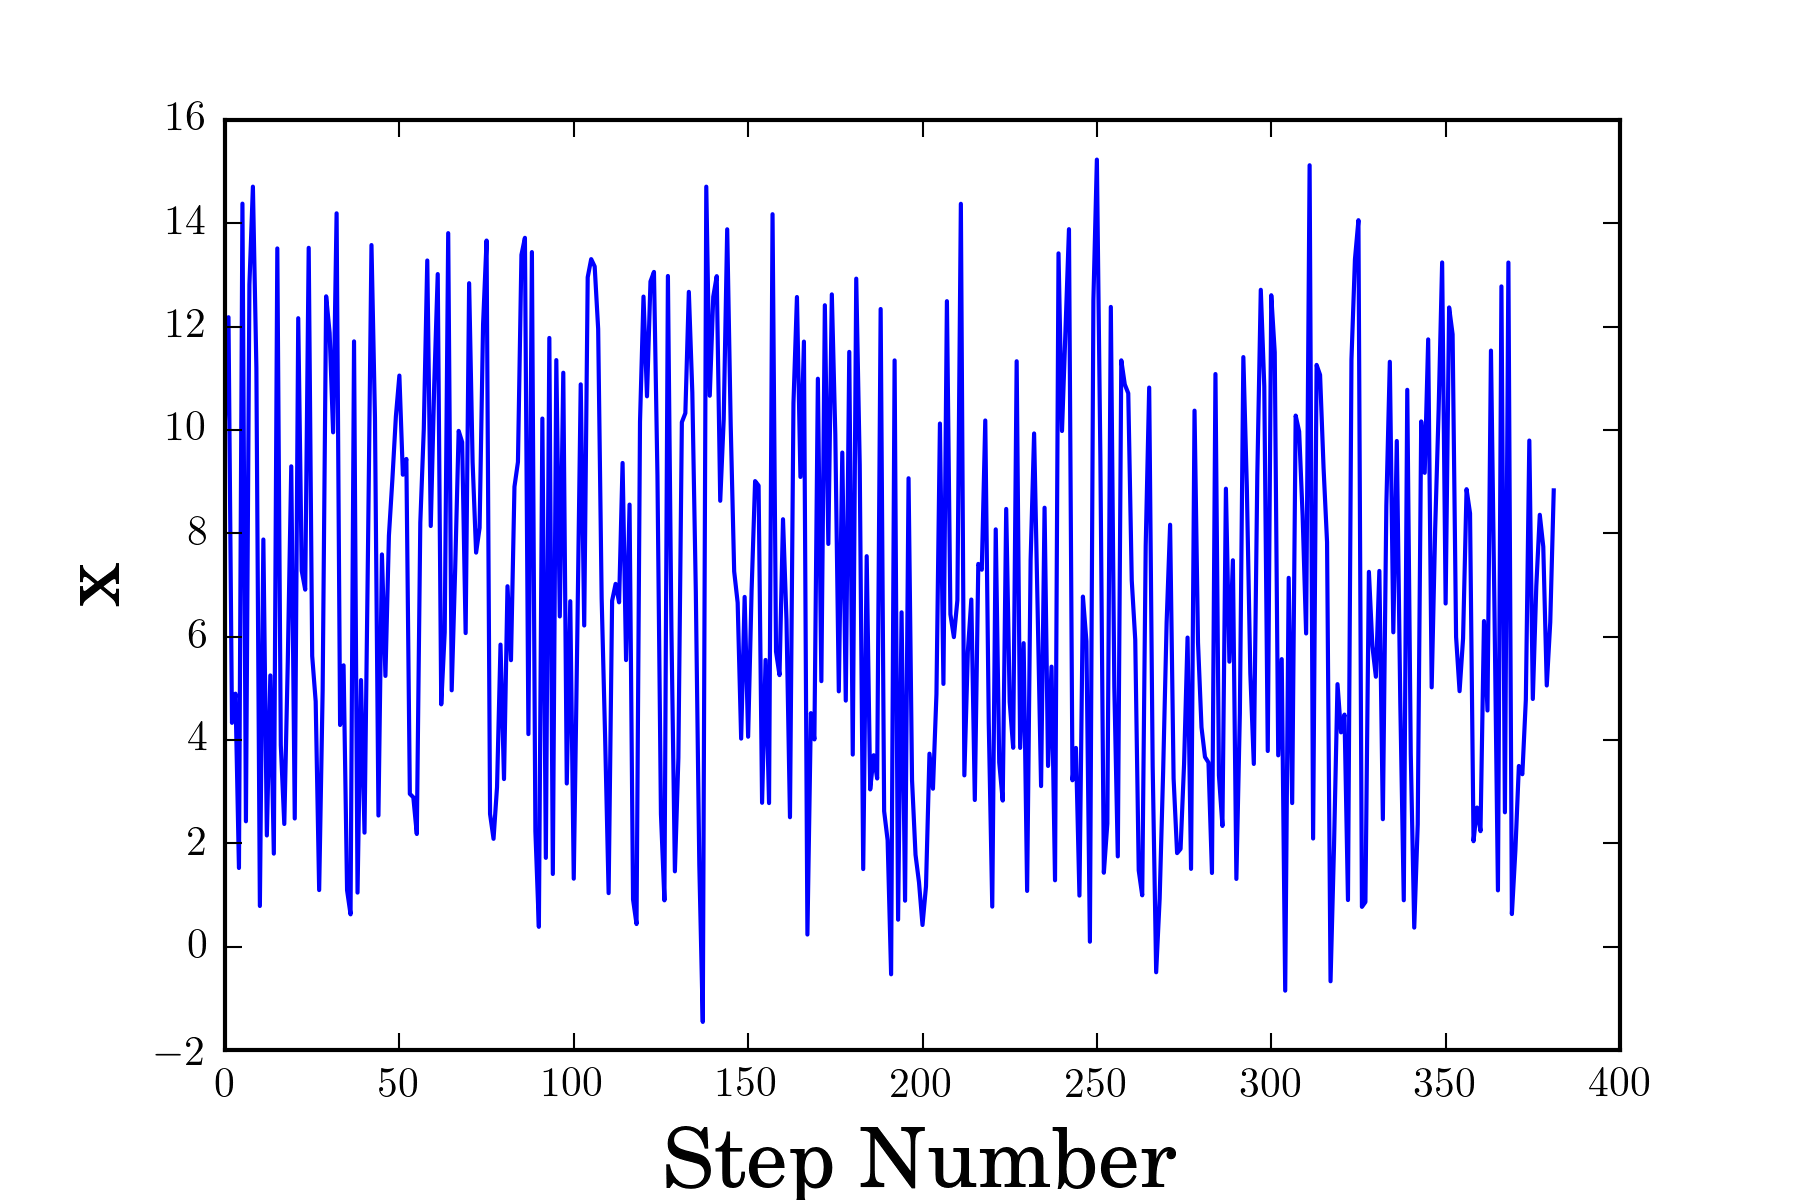
\includegraphics[width=\linewidth]{step_vs_x_mcmc.png}
  \caption{x vs. Step Number}
  \label{fig:sub1y}
\end{subfigure}%
\begin{subfigure}{0.5\textwidth}
  \centering
  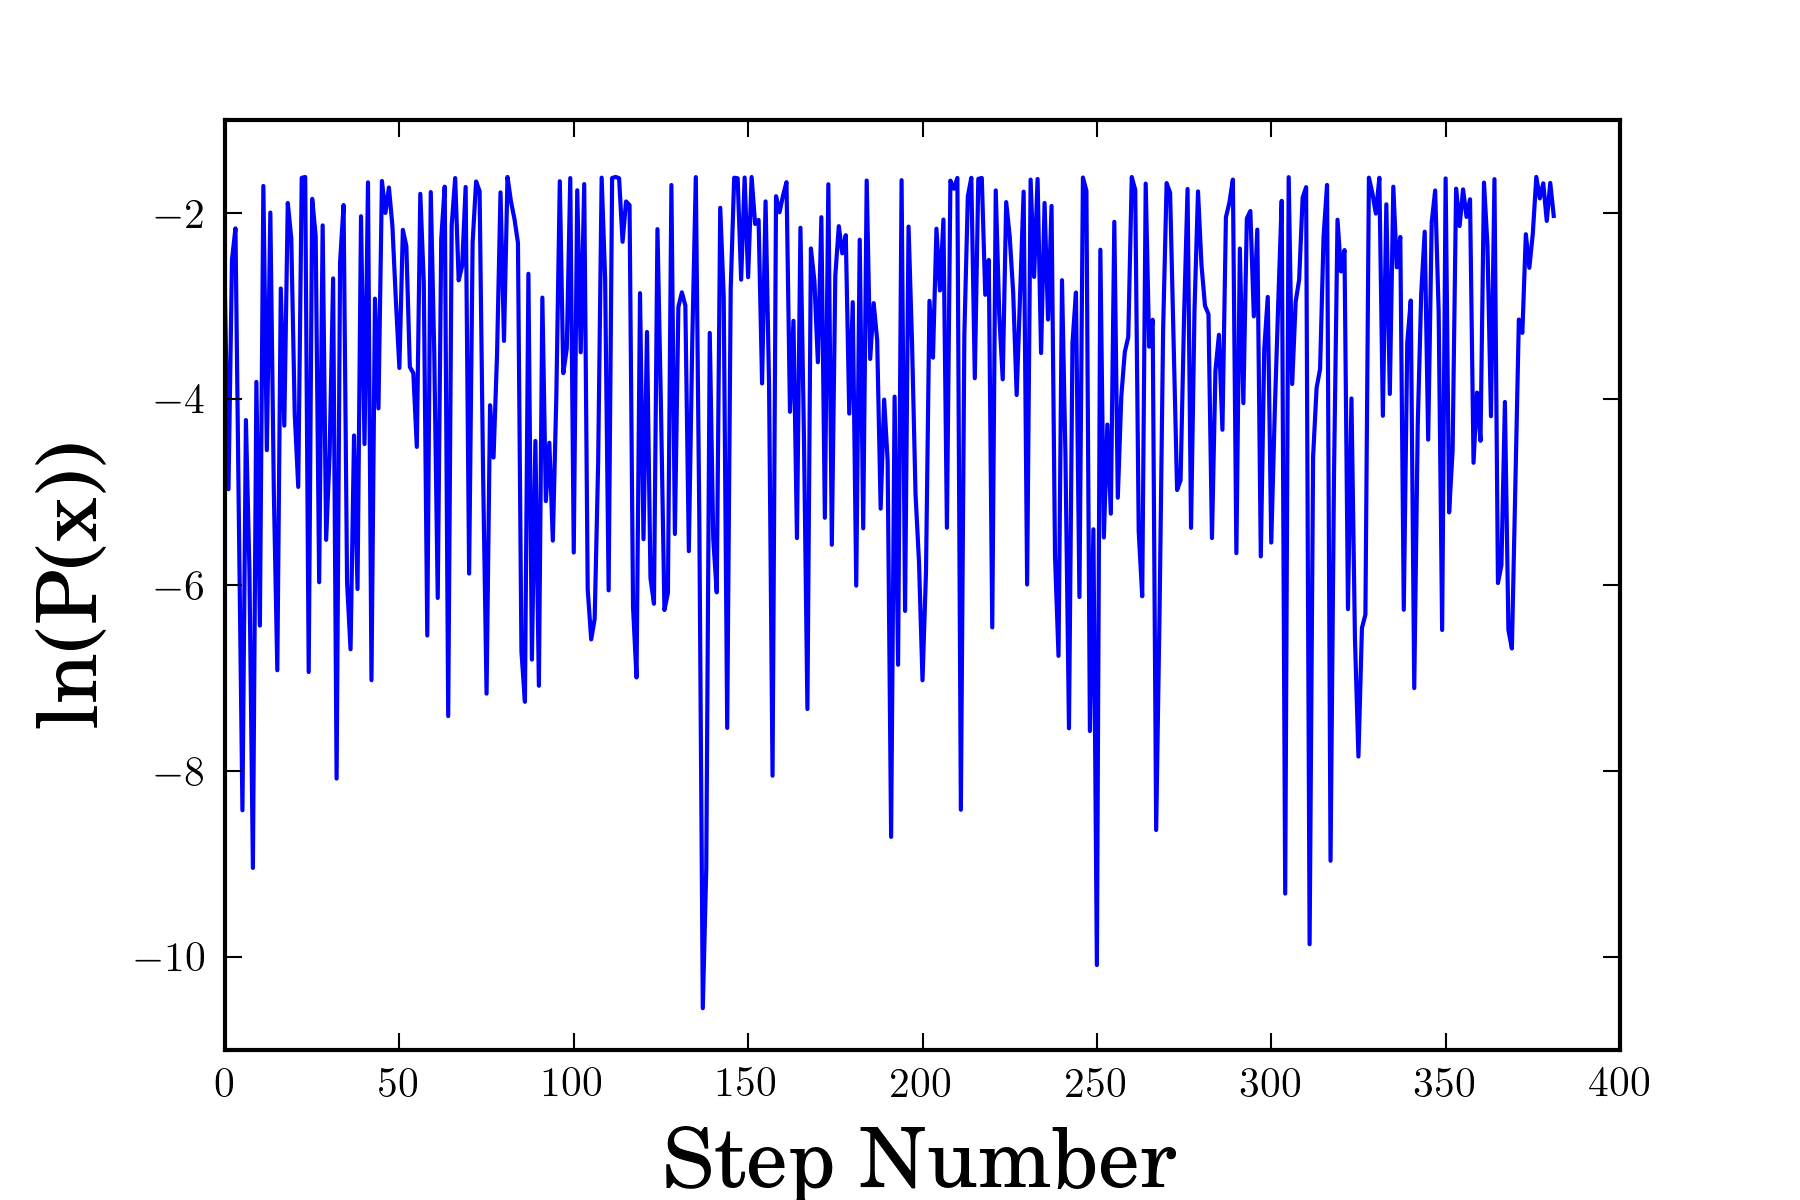
\includegraphics[width=\linewidth]{lnp_step_number_mcmc.png}
  \caption{ln(P(x) vs. Step Number}
  \label{fig:sub2y}
\end{subfigure}
\caption{These figures show the behavior of each of the steps in the MCMC chain.}
\label{fig:testy}
\end{figure}

The figures above look how one would expect, with a fairly uniform distribution and no bulk trends that are clearly visible by eye. This indicates that the sampler has likely converged.


\begin{figure}[H]
\centering
\begin{subfigure}{.5\textwidth}
  \centering
  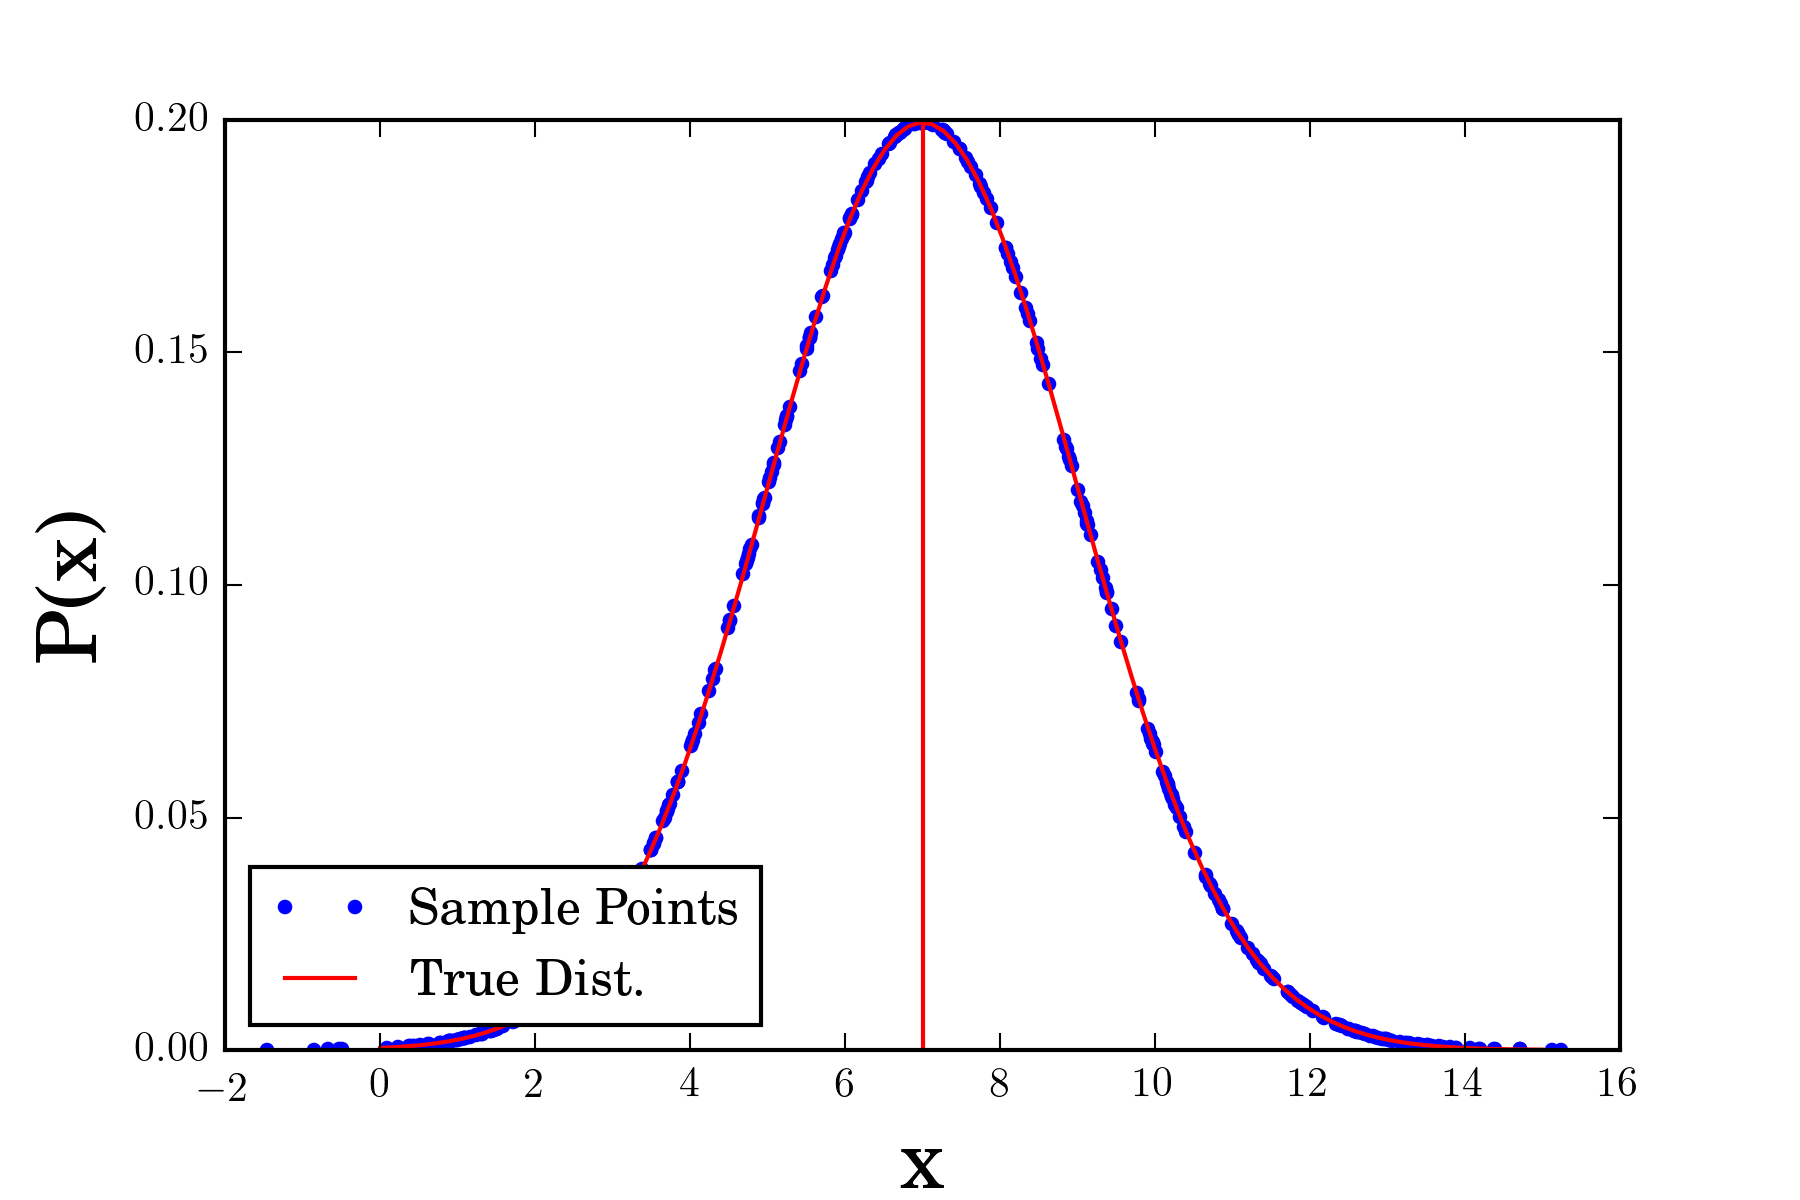
\includegraphics[width=\linewidth]{p_x_mcmc_true.png}
  \caption{P(x) vs. x}
  \label{fig:sub1}
\end{subfigure}%
\begin{subfigure}{0.5\textwidth}
  \centering
  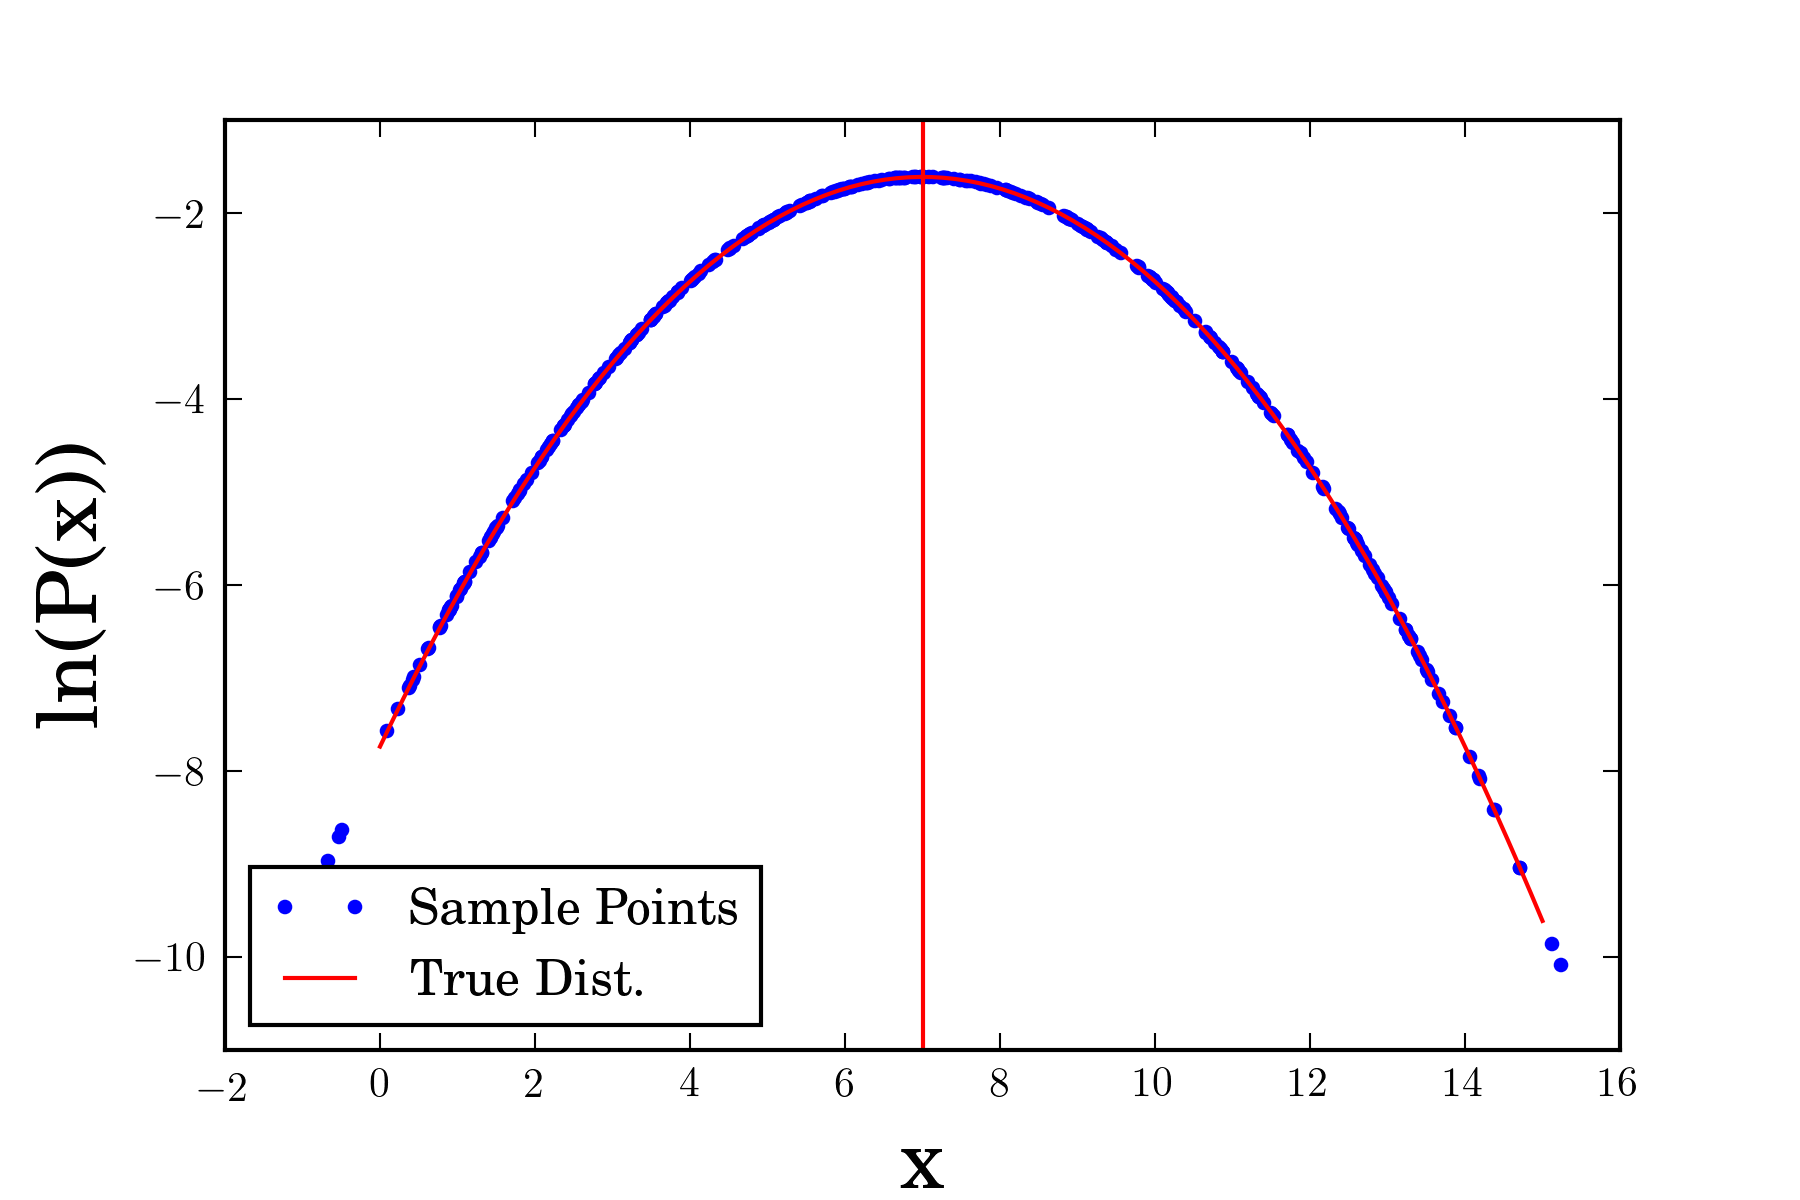
\includegraphics[width=\linewidth]{lnp_x_true_mcmc.png}
  \caption{ln(P(x) vs. x}
  \label{fig:sub2}
\end{subfigure}
\caption{These two plots compare the sampled posterior with the true distribution for both P(x) and ln(P(x)).}
\label{fig:test}
\end{figure}
 The red vertical lines denote the true mean, 7, and the red curves denote the real distribution. As evidenced by the plots, the sampler closely follows the posterior distribution.

\section*{Problem 3}

\textit{Using a probabilistic framework, write code that fits a straight line to fake data. You will need to write a function that simulates fake data that includes Gaussian noise and an arbitrary number of points.}

\subsection*{a.}
\textit{Assume true values of m=5, b=-2. Use the M-H MCMC sampler you wrote in problem 2 to infer the true values of m and b for 10, 100, 1000 data points. Choose a modest amplitude for your uncertainties and clearly indicate your choice. For simplicity, you may assume a top hat ('flat') priors for m and b. Make relevant diagnostic plots to indicate convergence, and plot your final results using corner.py.}

I coded this in a python notebook called ps1\_p3.ipynb.

For this problem I began by simulating fake linear data with Gaussian errors, sampled from a Gaussian centered at 0 with a standard deviation of 2. 
I begin with an initial value for m and b of 0. I then find a new value of m and b from a Gaussian centered at the previous values of m and b with a standard deviation of 20. This standard deviation was chosen through trial and error to yield a desirable acceptance rate. In order to check whether to shift to the new values of m and b I square the differences between each fake data point y and the theoretical value with said m and b using fake data point x . I sum these values and return the reciprocal of this value as my P(m,b) because I want to step towards the minimum of this quantity. The rest of the process, which includes building my chain while moving through difference m and b values proceeds in the same way as my previous MCMC chain.

Below is a plot of 100 fake data points with error bars.

\begin{figure}[H]
\centering
\caption{100 Fake Data Points}
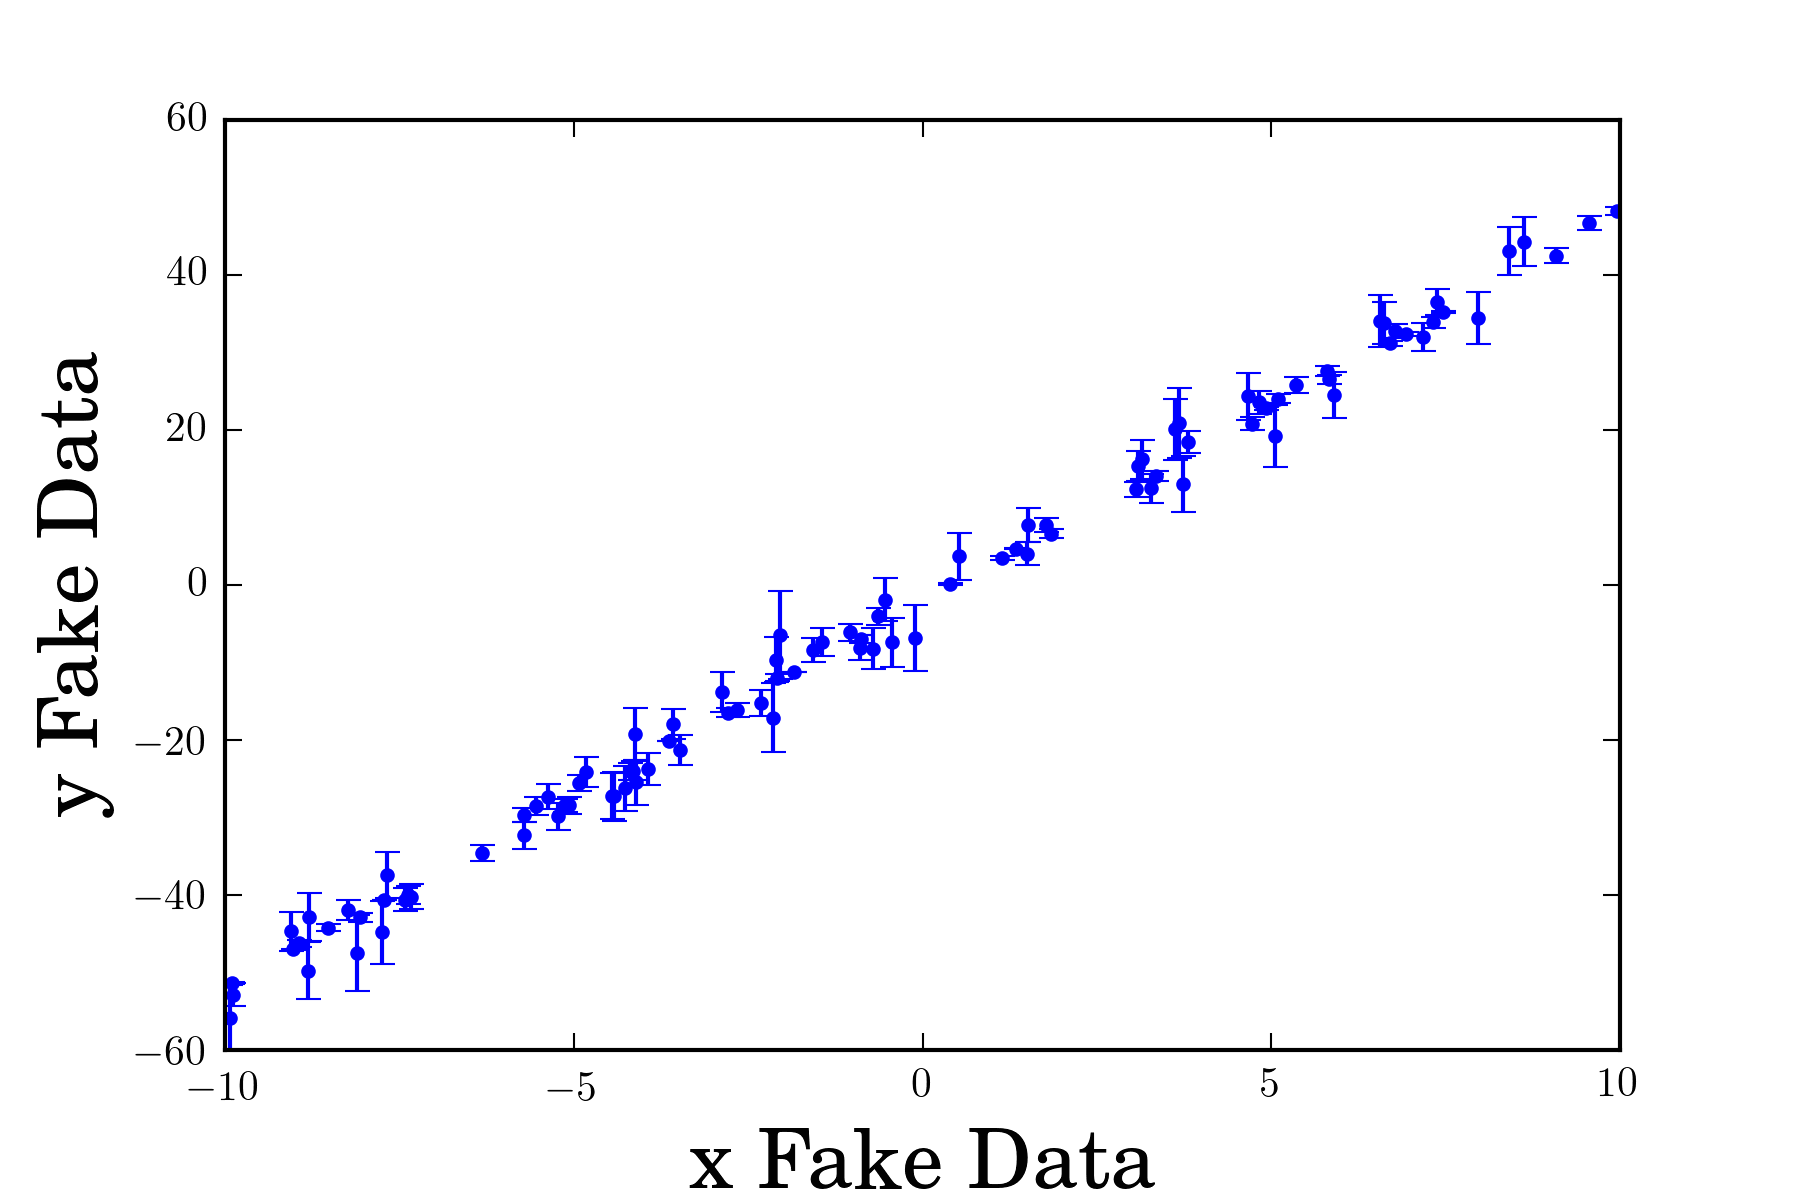
\includegraphics[scale = 0.6]{x_y_100_fake_data_points.png}
\end{figure}

I ran my MCMC chain 3 times, for 10, 100 and 1000 fake data points. Below are the plots of ln(P) vs. Step Number, Slope (m) and Intercept (b) for all three trials. The red vertical line denotes the true value of m or b. I use 5000 steps for each chain. The acceptance ratio for the 10, 100, and 1000 point data sets were 0.41, 0.40 and 0.21, respectively.


\begin{figure}[H]
\caption{10 Fake Data Points}
\minipage{0.32\textwidth}
  \includegraphics[width=\linewidth]{lnp_step_10_data_pts.png}
  %\caption*{}\label{fig:awesome_image1}
\endminipage\hfill
\minipage{0.32\textwidth}
  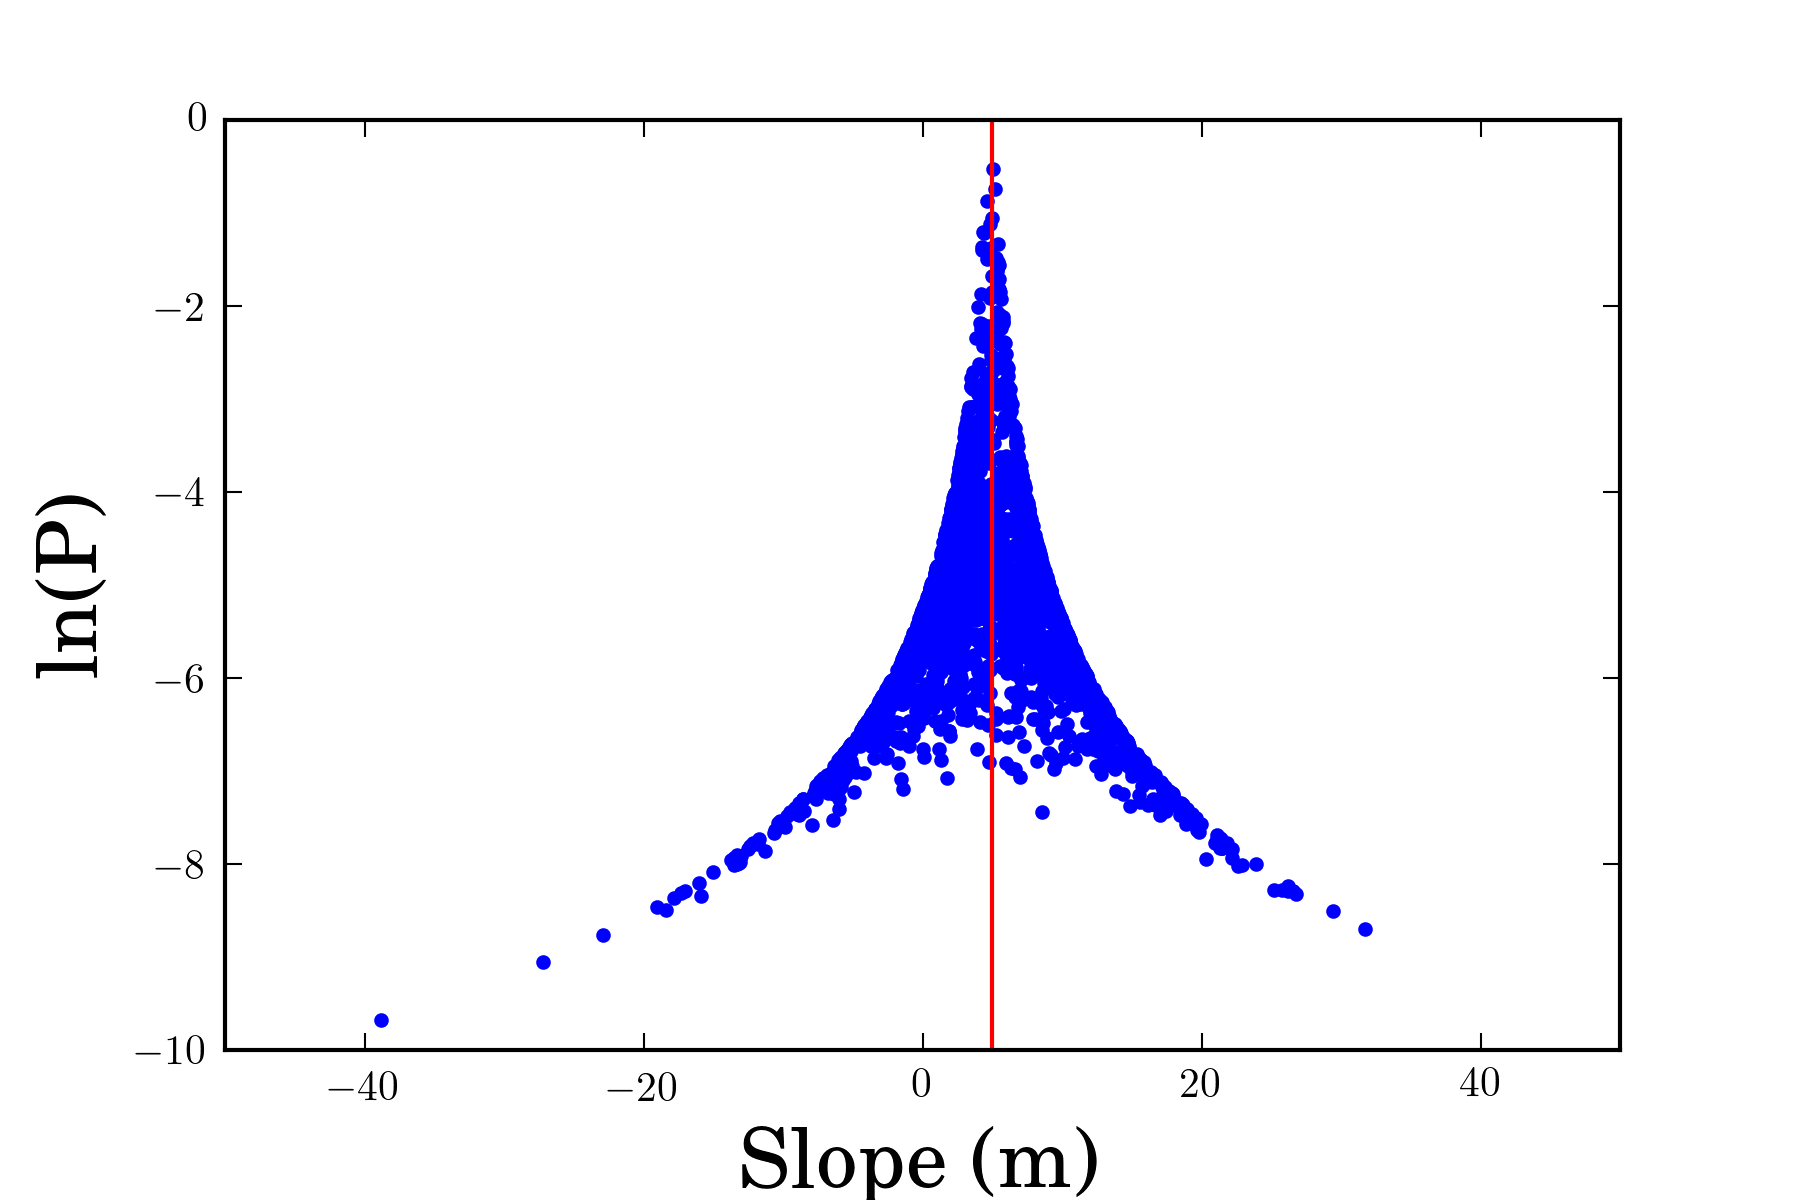
\includegraphics[width=\linewidth]{lnp_m_10_data_points.png}
  %\caption*{    Figure 3: 10 Fake Data Points}\label{fig:awesome_image2}
\endminipage\hfill
\minipage{0.32\textwidth}%
  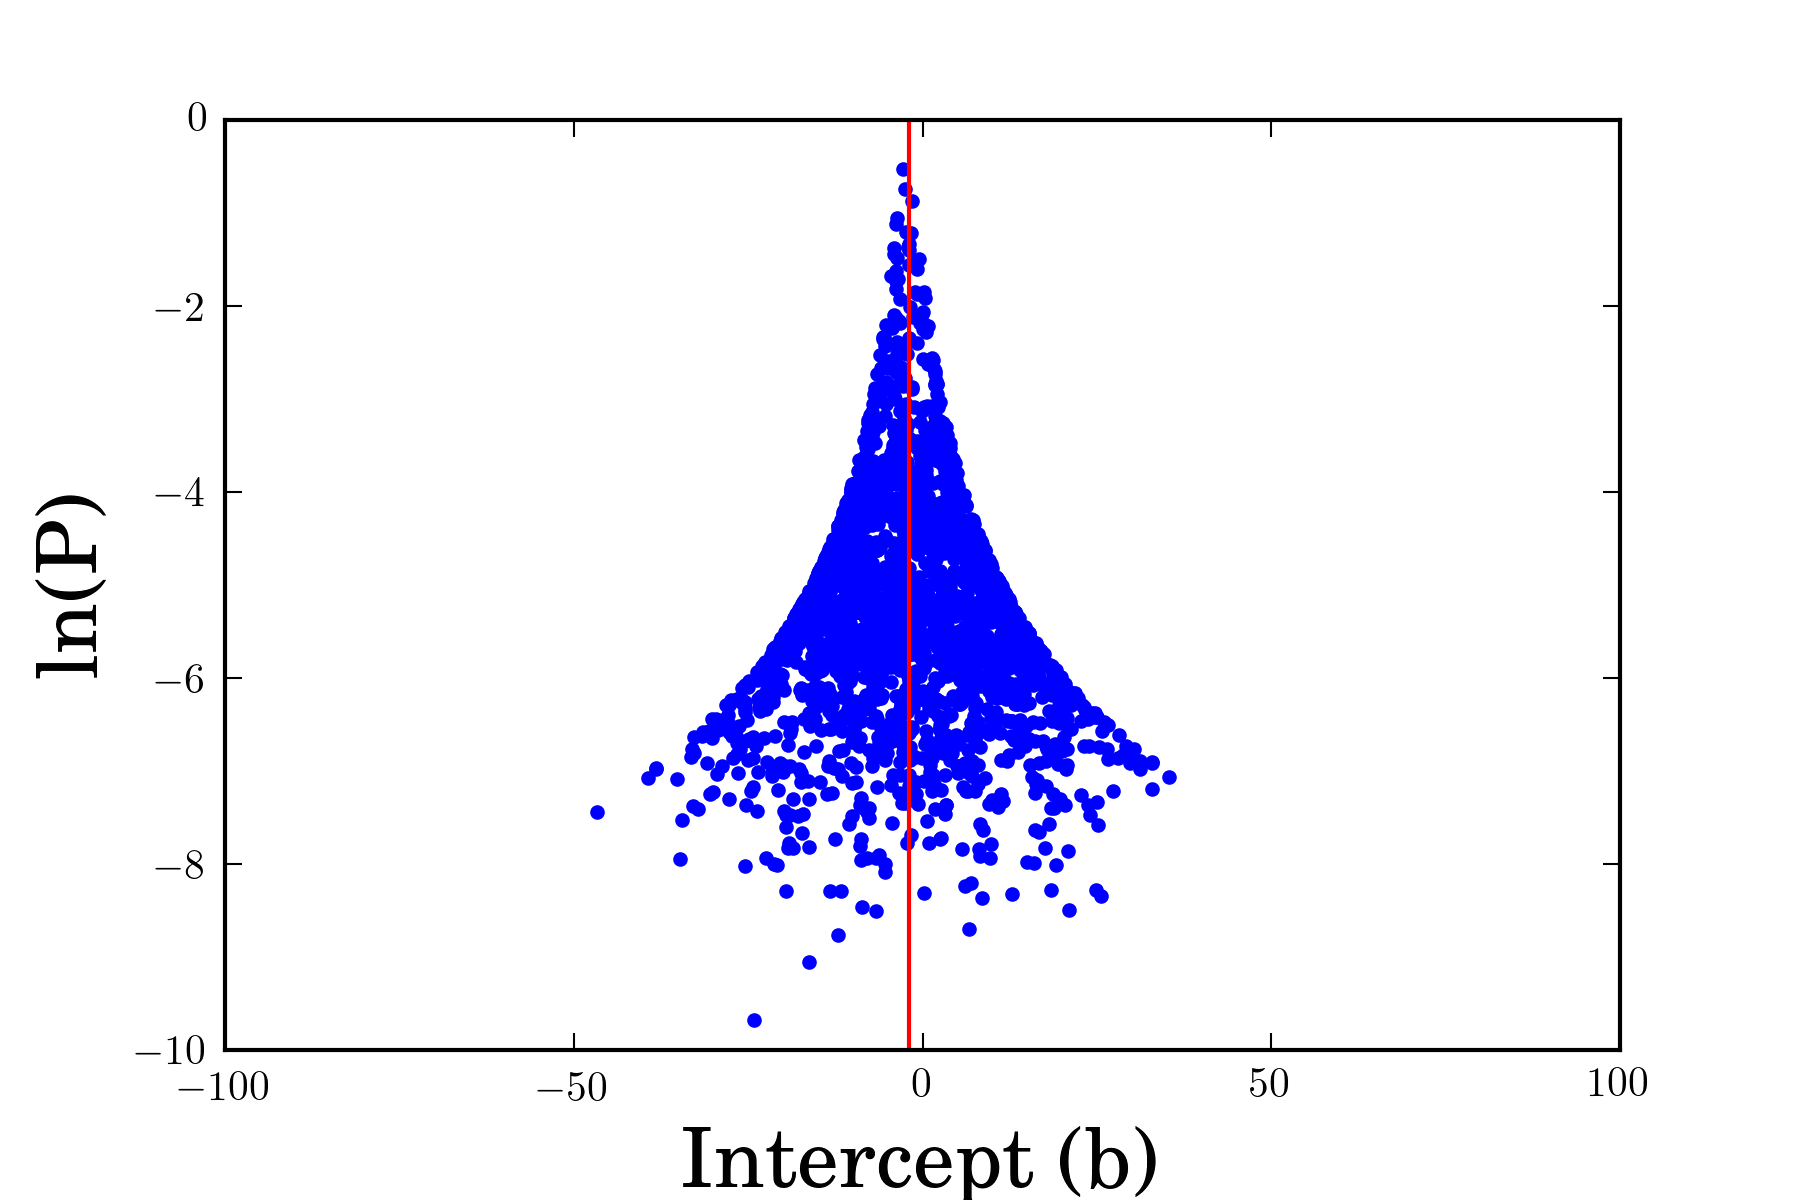
\includegraphics[width=\linewidth]{lnp_b_10_data_points.png}
  %\caption*{}\label{fig:awesome_image3}
\endminipage\hfill
\end{figure}

\begin{figure}[H]
\caption{100 Fake Data Points}
\minipage{0.32\textwidth}
  \includegraphics[width=\linewidth]{lnp_step_100_data_pts.png}
\endminipage\hfill
\minipage{0.32\textwidth}
  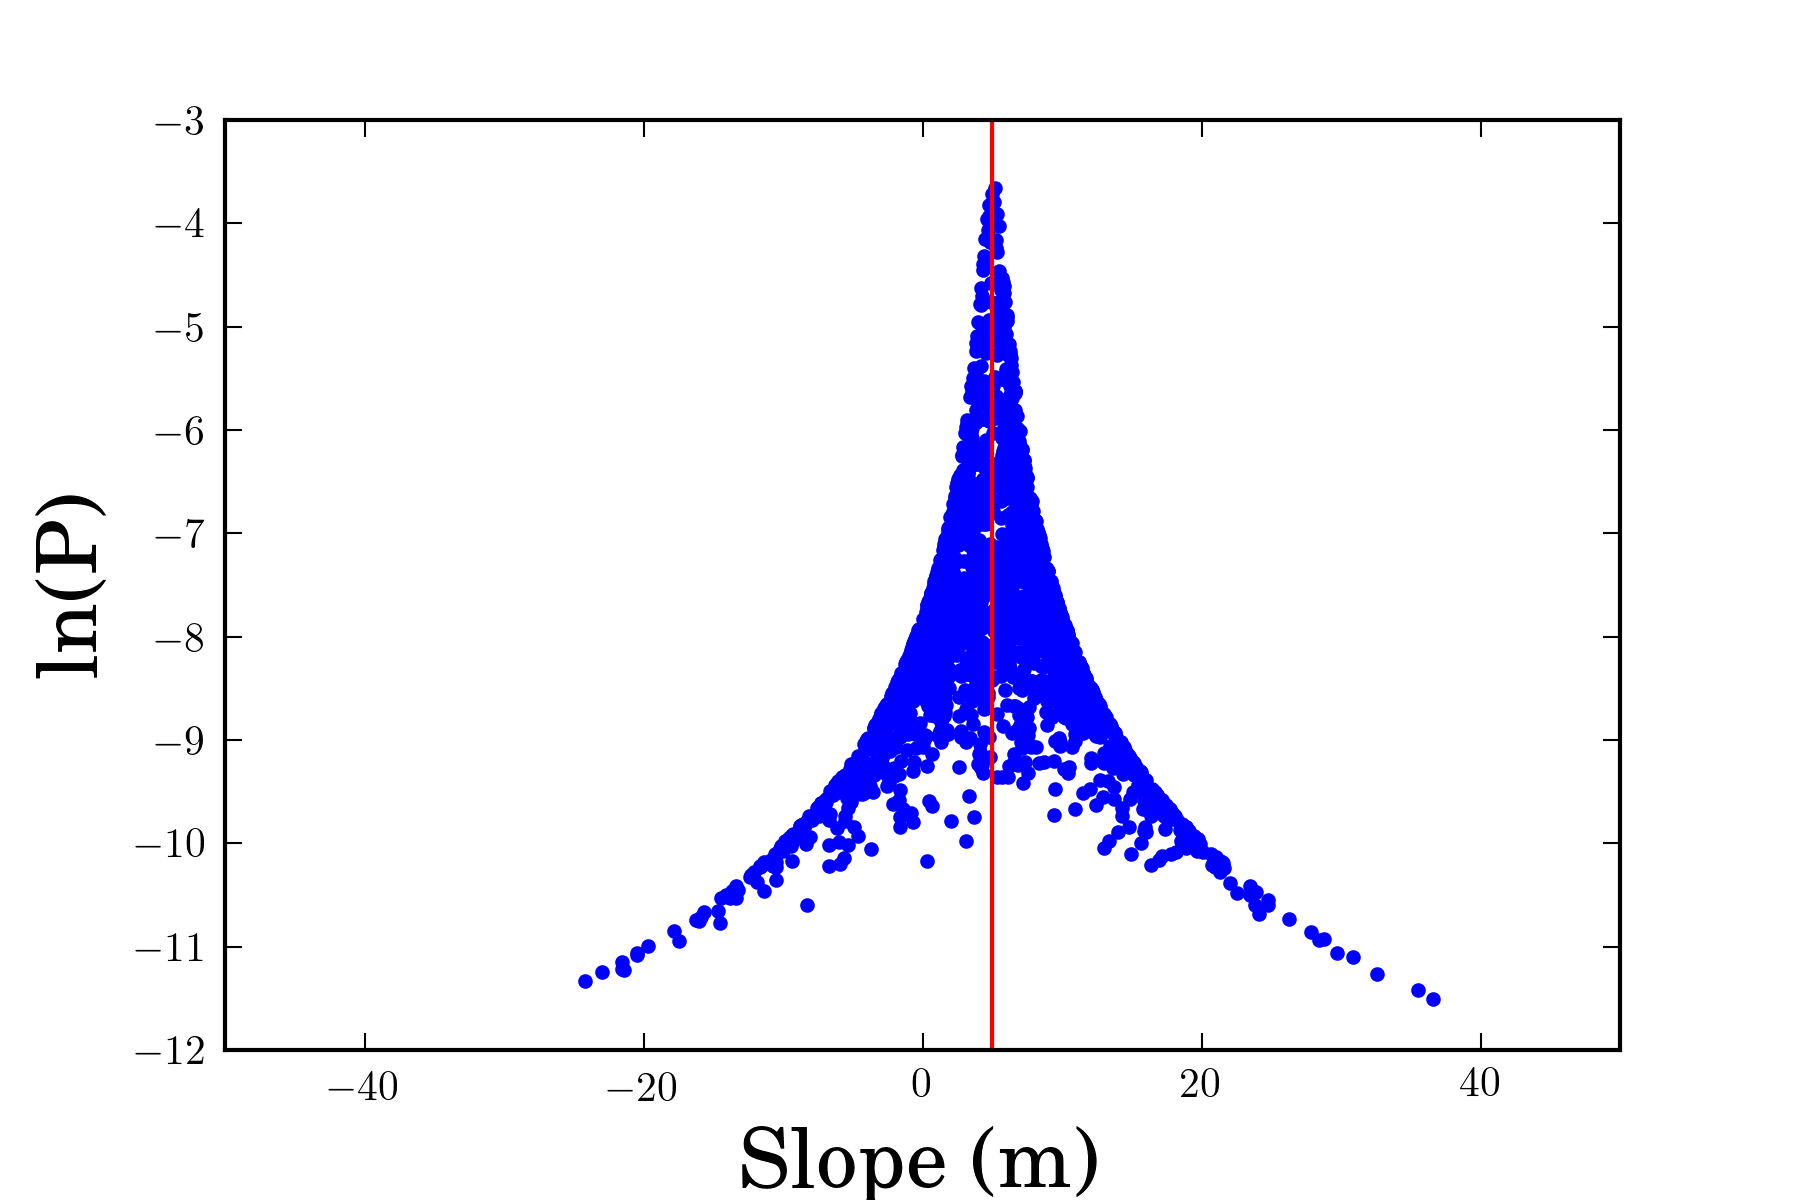
\includegraphics[width=\linewidth]{lnp_m_100_data_points.png}
\endminipage\hfill
\minipage{0.32\textwidth}%
  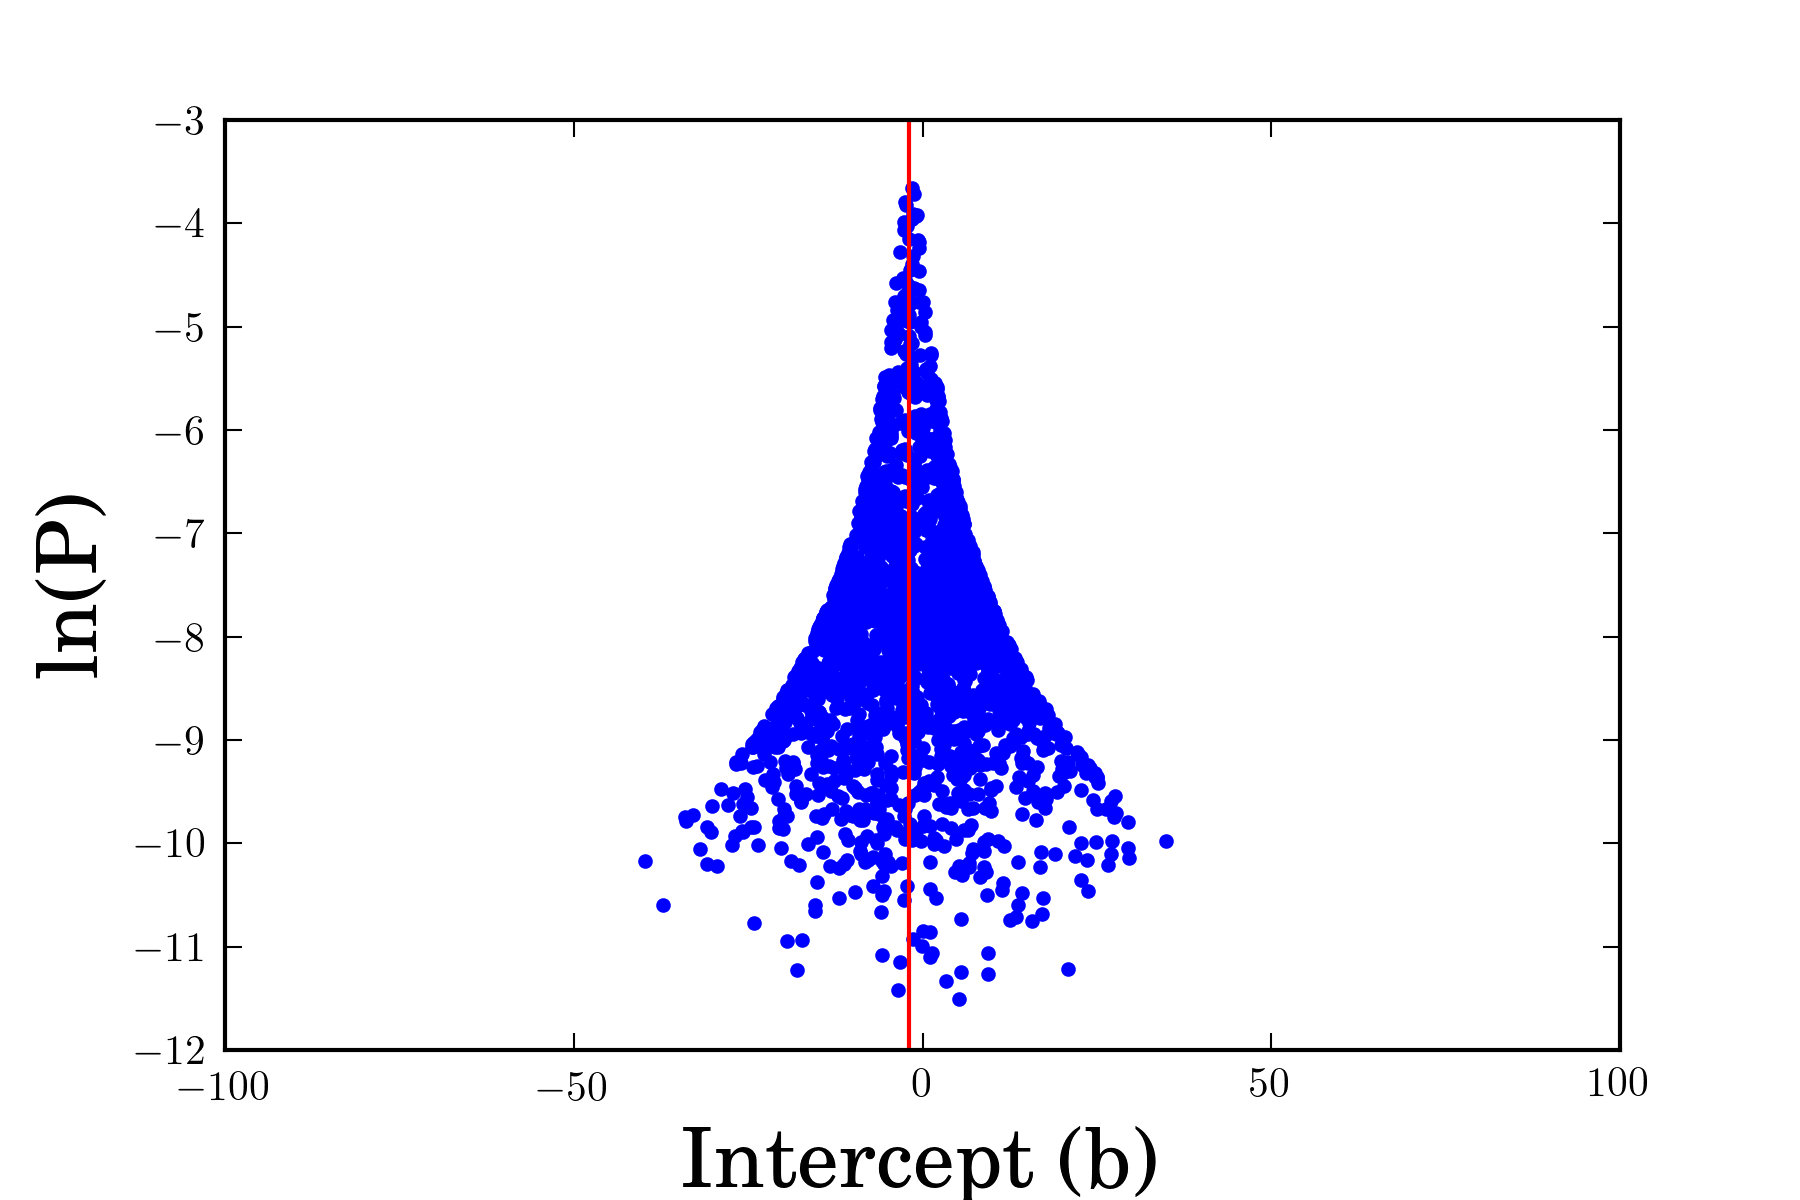
\includegraphics[width=\linewidth]{lnp_b_100_data_points.png}
\endminipage\hfill
\end{figure}

\begin{figure}[H]
\caption{1000 Fake Data Points}
\minipage{0.32\textwidth}
  \includegraphics[width=\linewidth]{lnp_step_1000_data_pts.png}
\endminipage\hfill
\minipage{0.32\textwidth}
  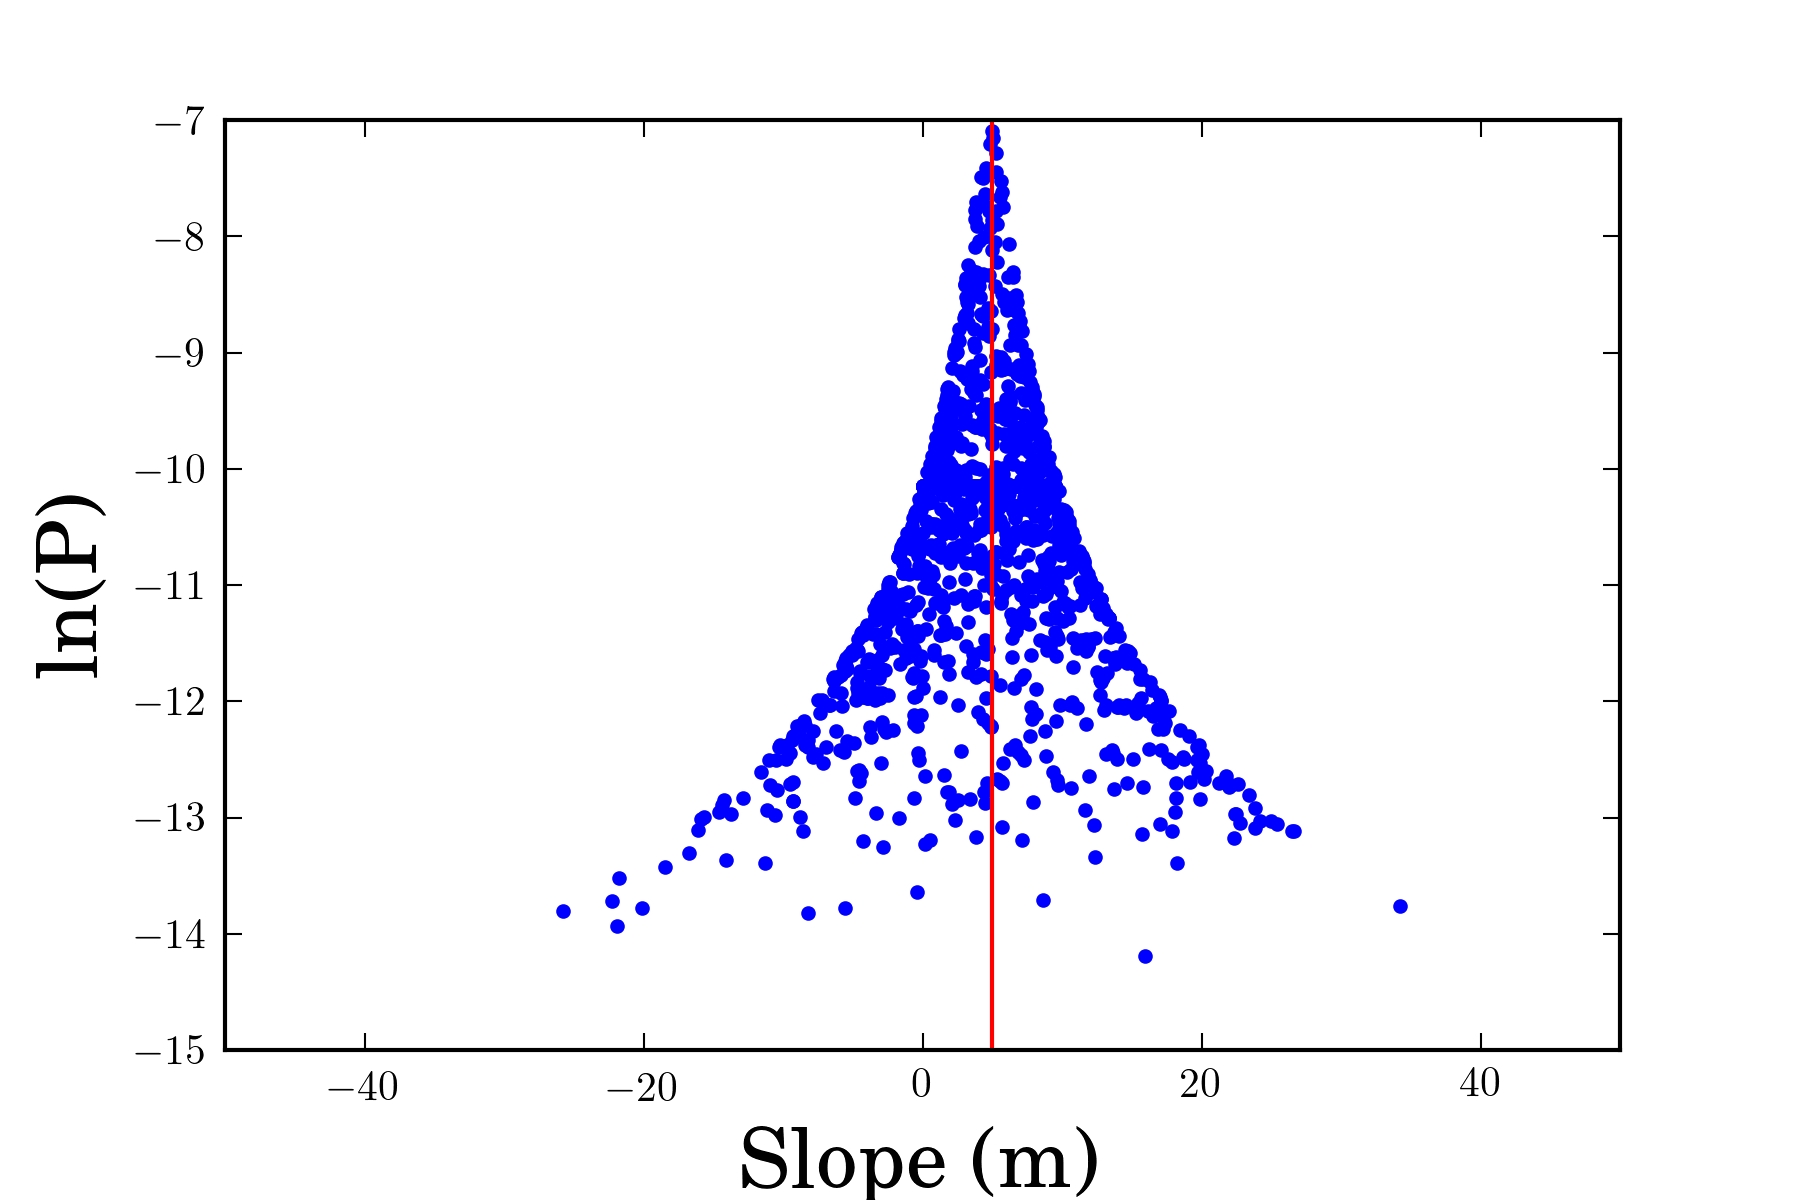
\includegraphics[width=\linewidth]{lnp_m_1000_data_points.png}
\endminipage\hfill
\minipage{0.32\textwidth}%
  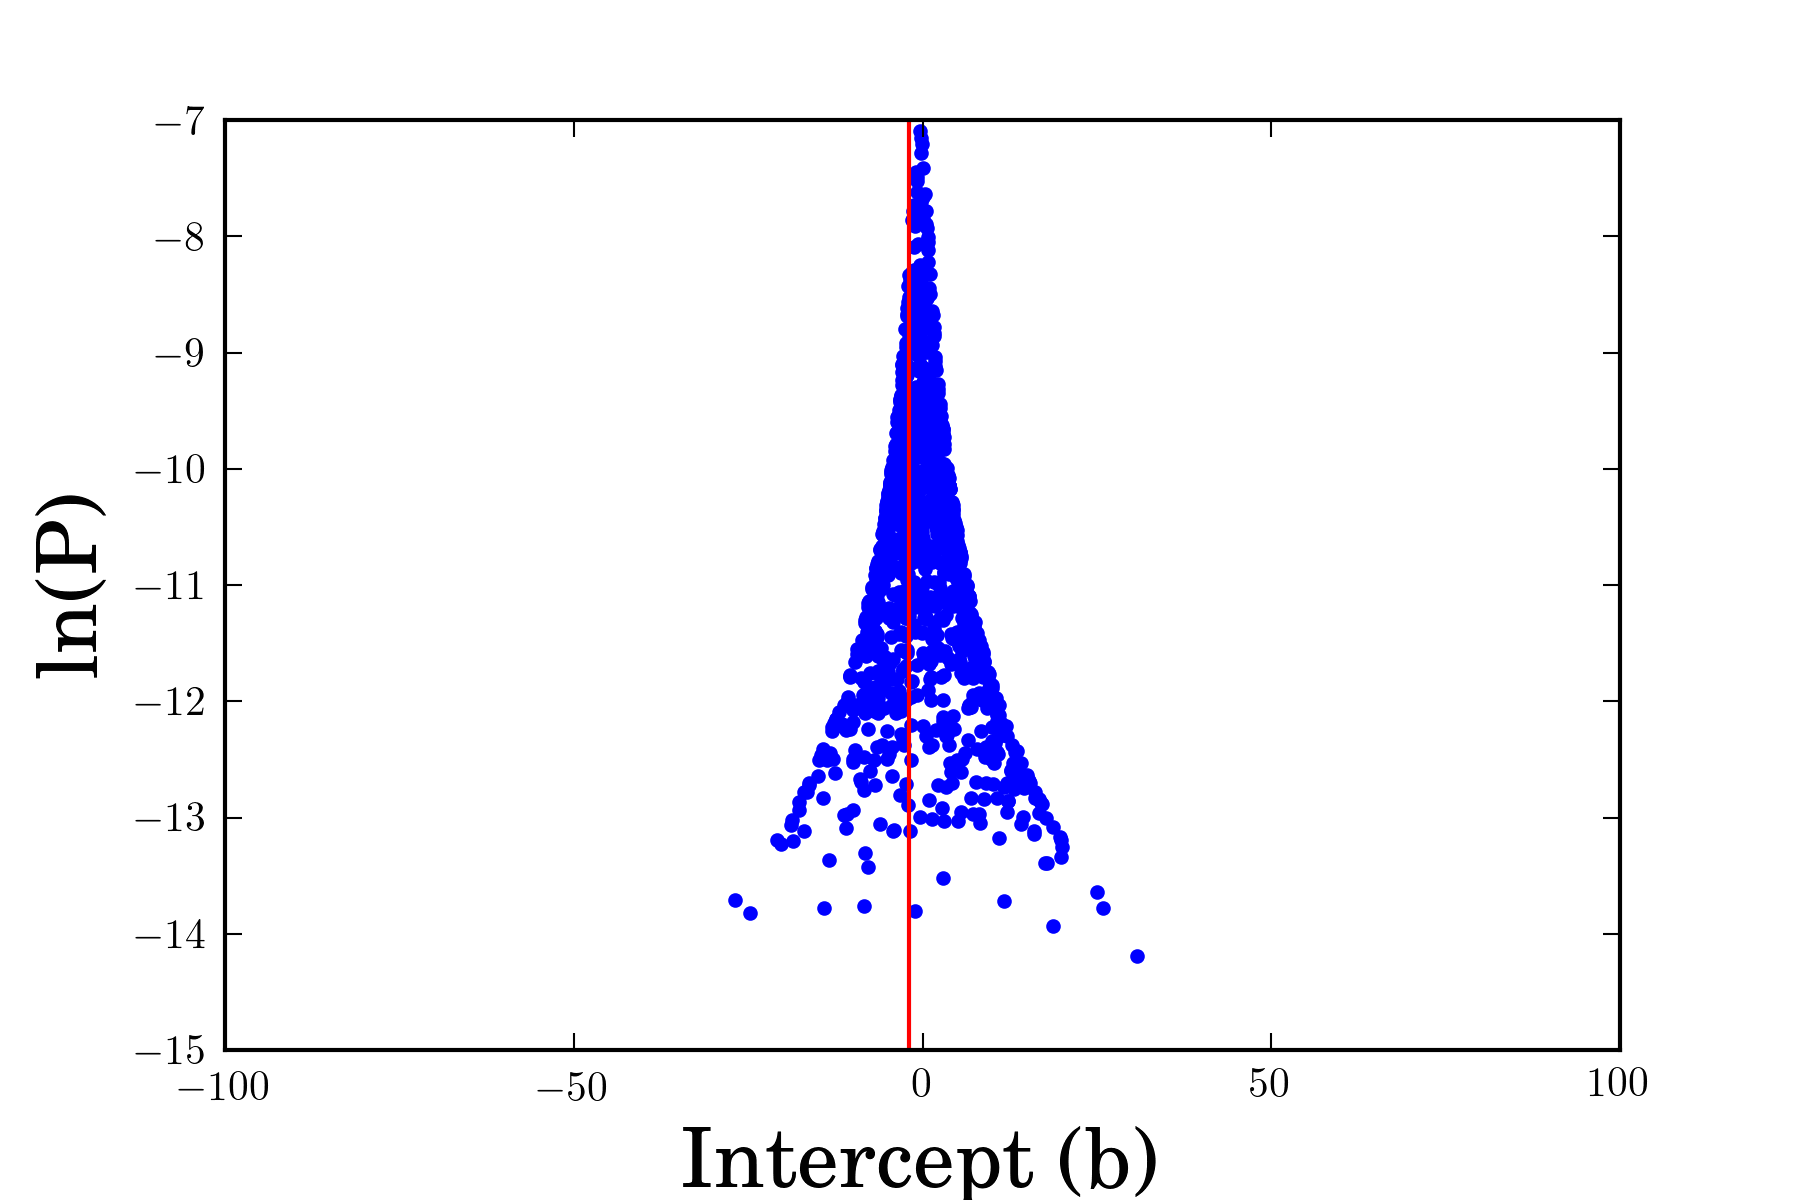
\includegraphics[width=\linewidth]{lnp_b_1000_data_points.png}
\endminipage\hfill
\end{figure}

Qualitatively, there doesn't seem to be significant differences caused by the number of fake data points. However, these plots do demonstrate that it is harder to fit the intercept than it is to fit the slope. Additionally, the Step Number vs. ln(P) plots don't show any clear trends, which indicates convergence. Also, the curves peak at the true values, which is expected.

Below are the contour plots for each data set size.


\begin{figure}[H]
\caption{Contour Plots for 10, 100, 1000 Fake Data Points (left to right)}
\minipage{0.32\textwidth}
  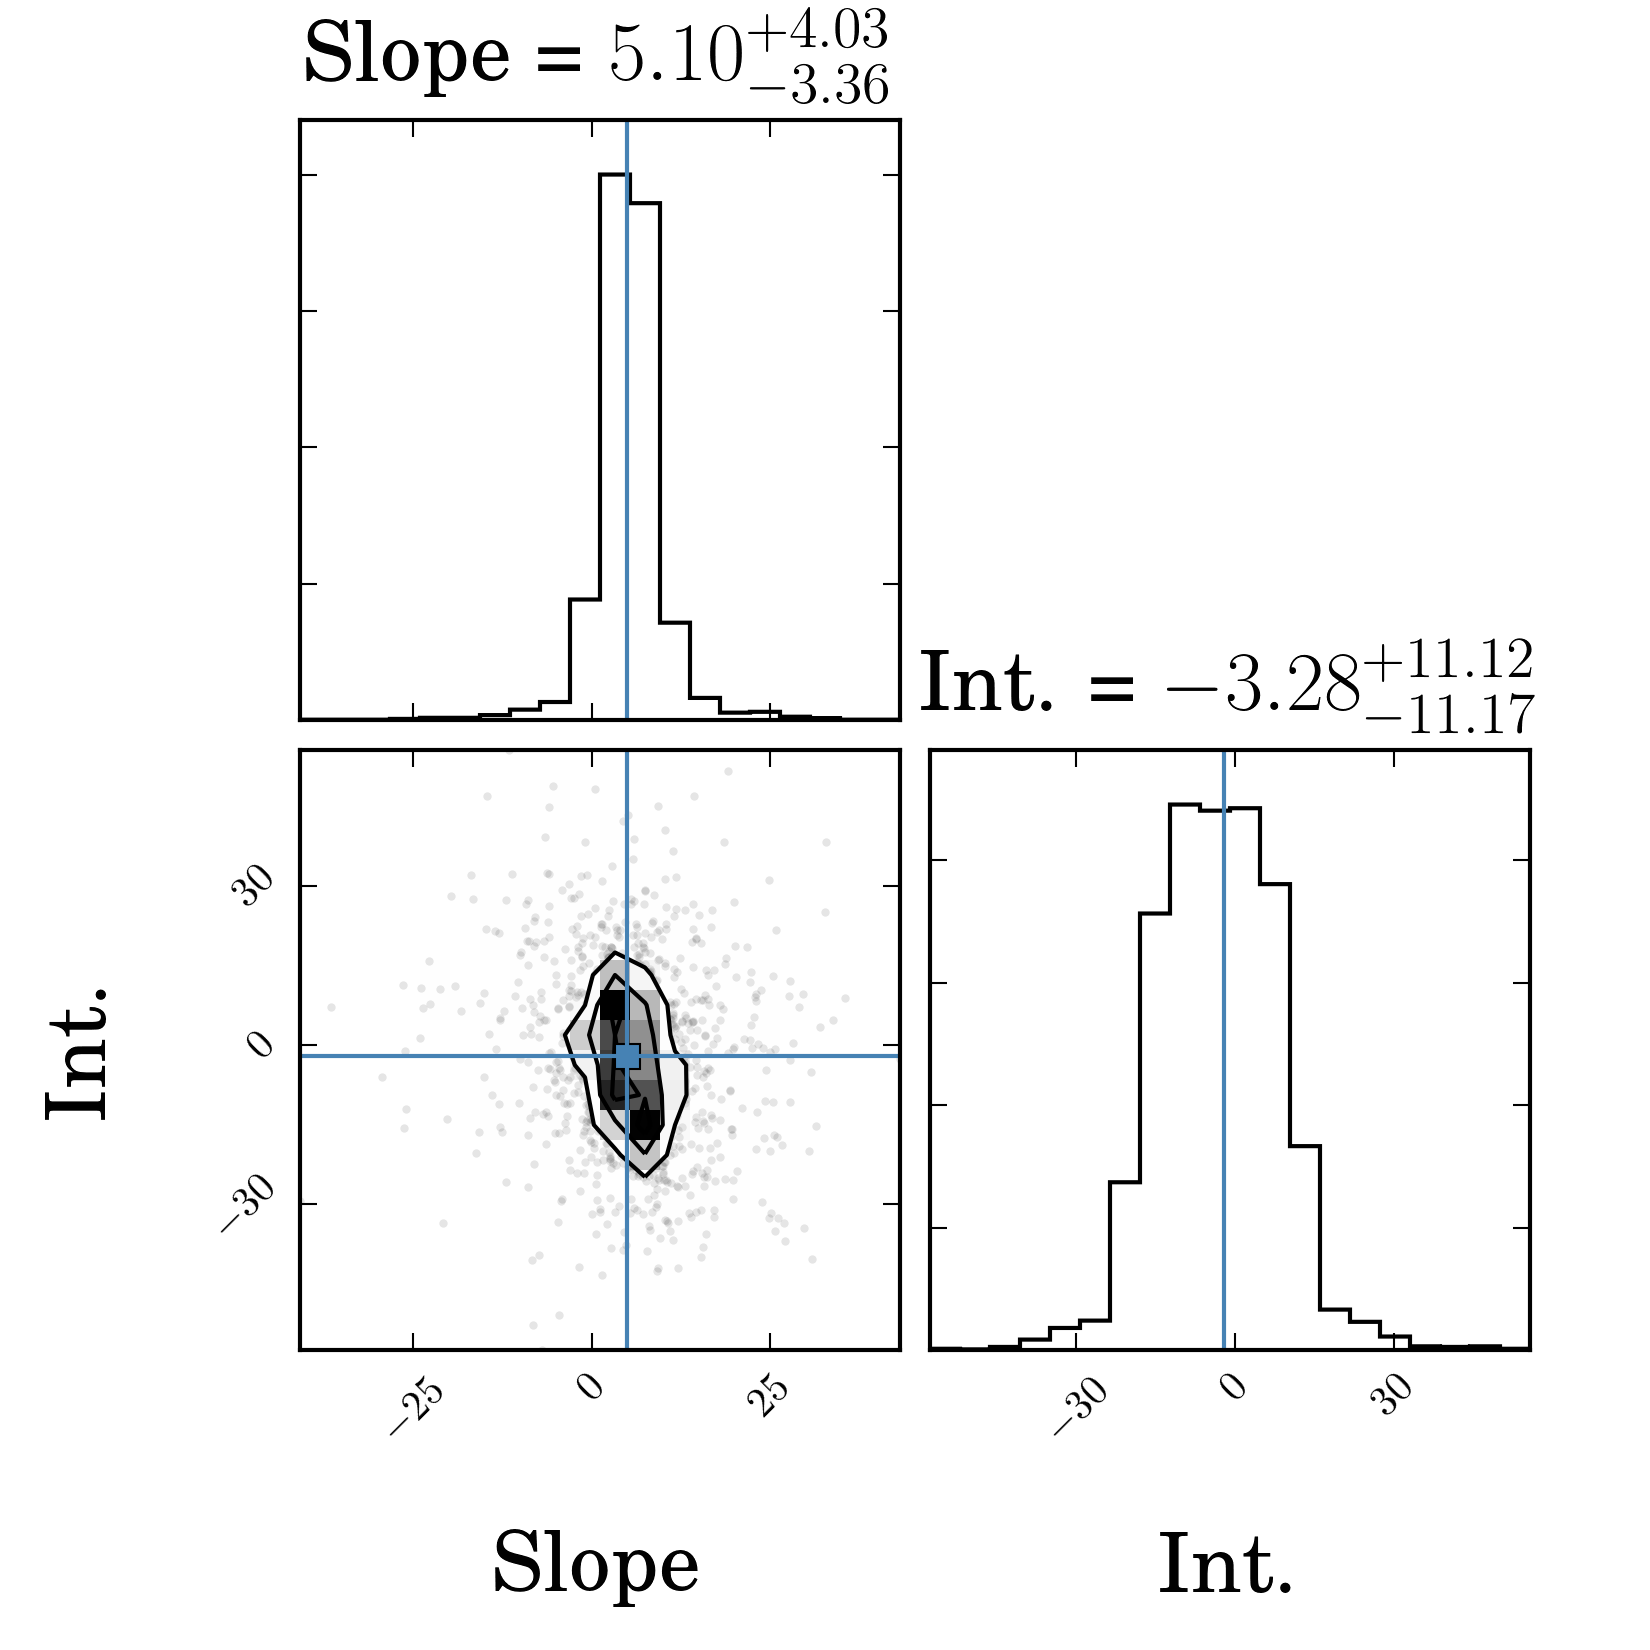
\includegraphics[width=\linewidth]{corner_10_data_points.png}
\endminipage\hfill
\minipage{0.32\textwidth}
  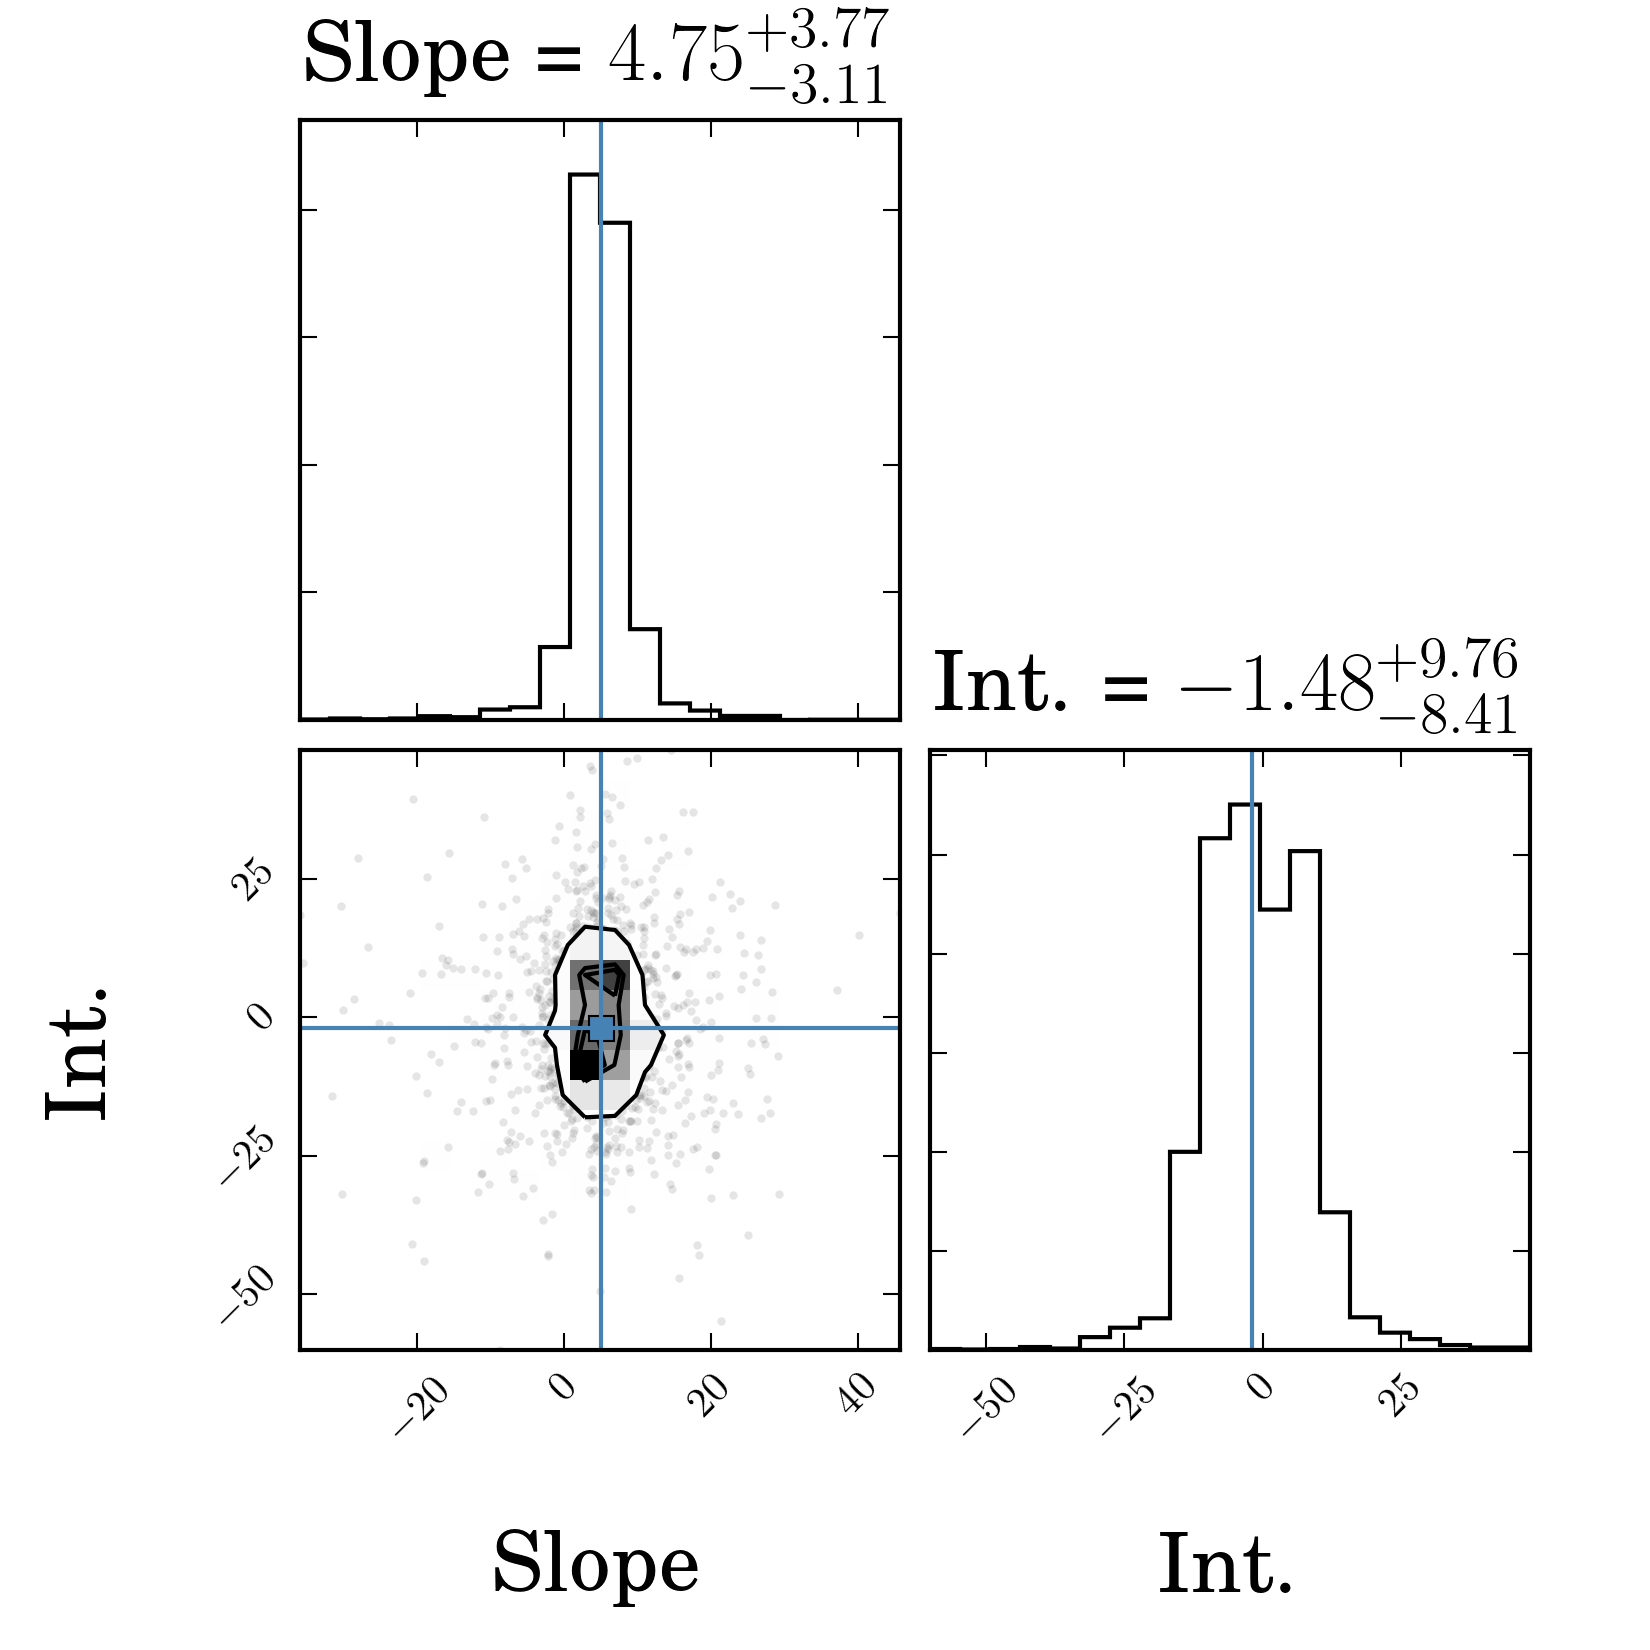
\includegraphics[width=\linewidth]{corner_100_data_points.png}
\endminipage\hfill
\minipage{0.32\textwidth}%
  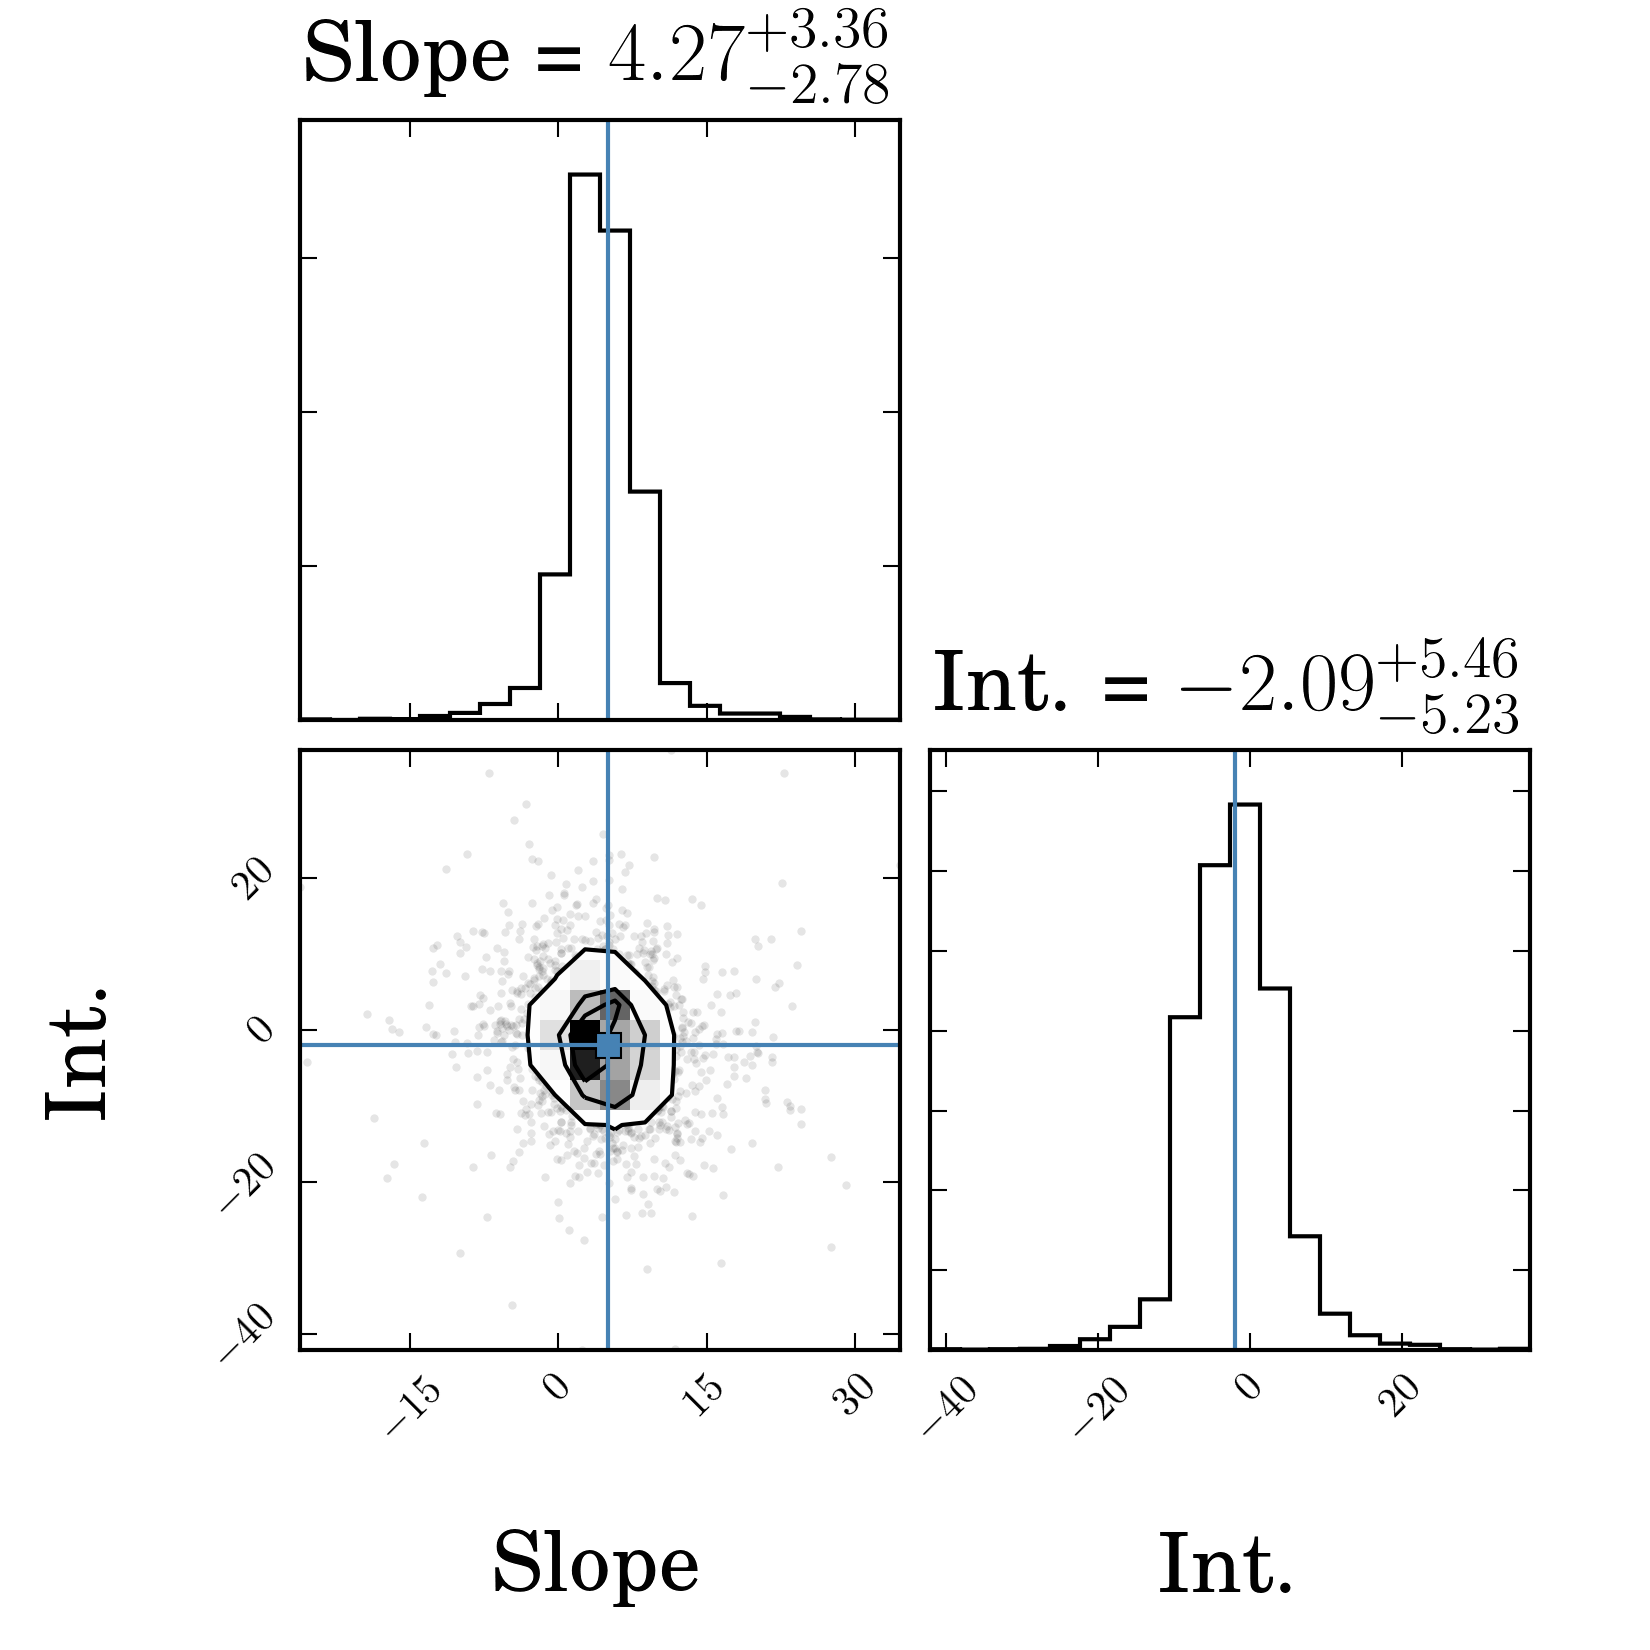
\includegraphics[width=\linewidth]{corner_1000_data_points.png}
\endminipage\hfill
\end{figure}

The posteriors of the intercept (b) value are consistently broader than the posterior of the slope (m). This arises from the fact that the slope is a much larger order effect because it is multiplied by each x value while the intercept is simply an added 1D translation. The elongation of the contour also demonstrates the greater uncertainty in b.  Additionally, the errors were larger for data sets with less values.

\subsection*{b.}
\textit{Repeat part (a), but replace your M-H sampler with emcee.}\\
After coding up my own algorithm to find values of m and b, I used an MCMC software package called emcee. For this, I was able to use multiple walkers (I chose 100). Emcee definitely found more precise and accurate values of m and b for all three datasets, the 10, 100 and 1000 fake data points. The code for using emcee is included in my python notebook for part a. ( ps1\_p3.ipynb).

Below are the contour plots using corner.corner for 10, 100 and 1000 fake data points.

\begin{figure}[H]
\caption{Contour Plots for 10, 100, 1000 Fake Data Points (left to right)}
\minipage{0.32\textwidth}
  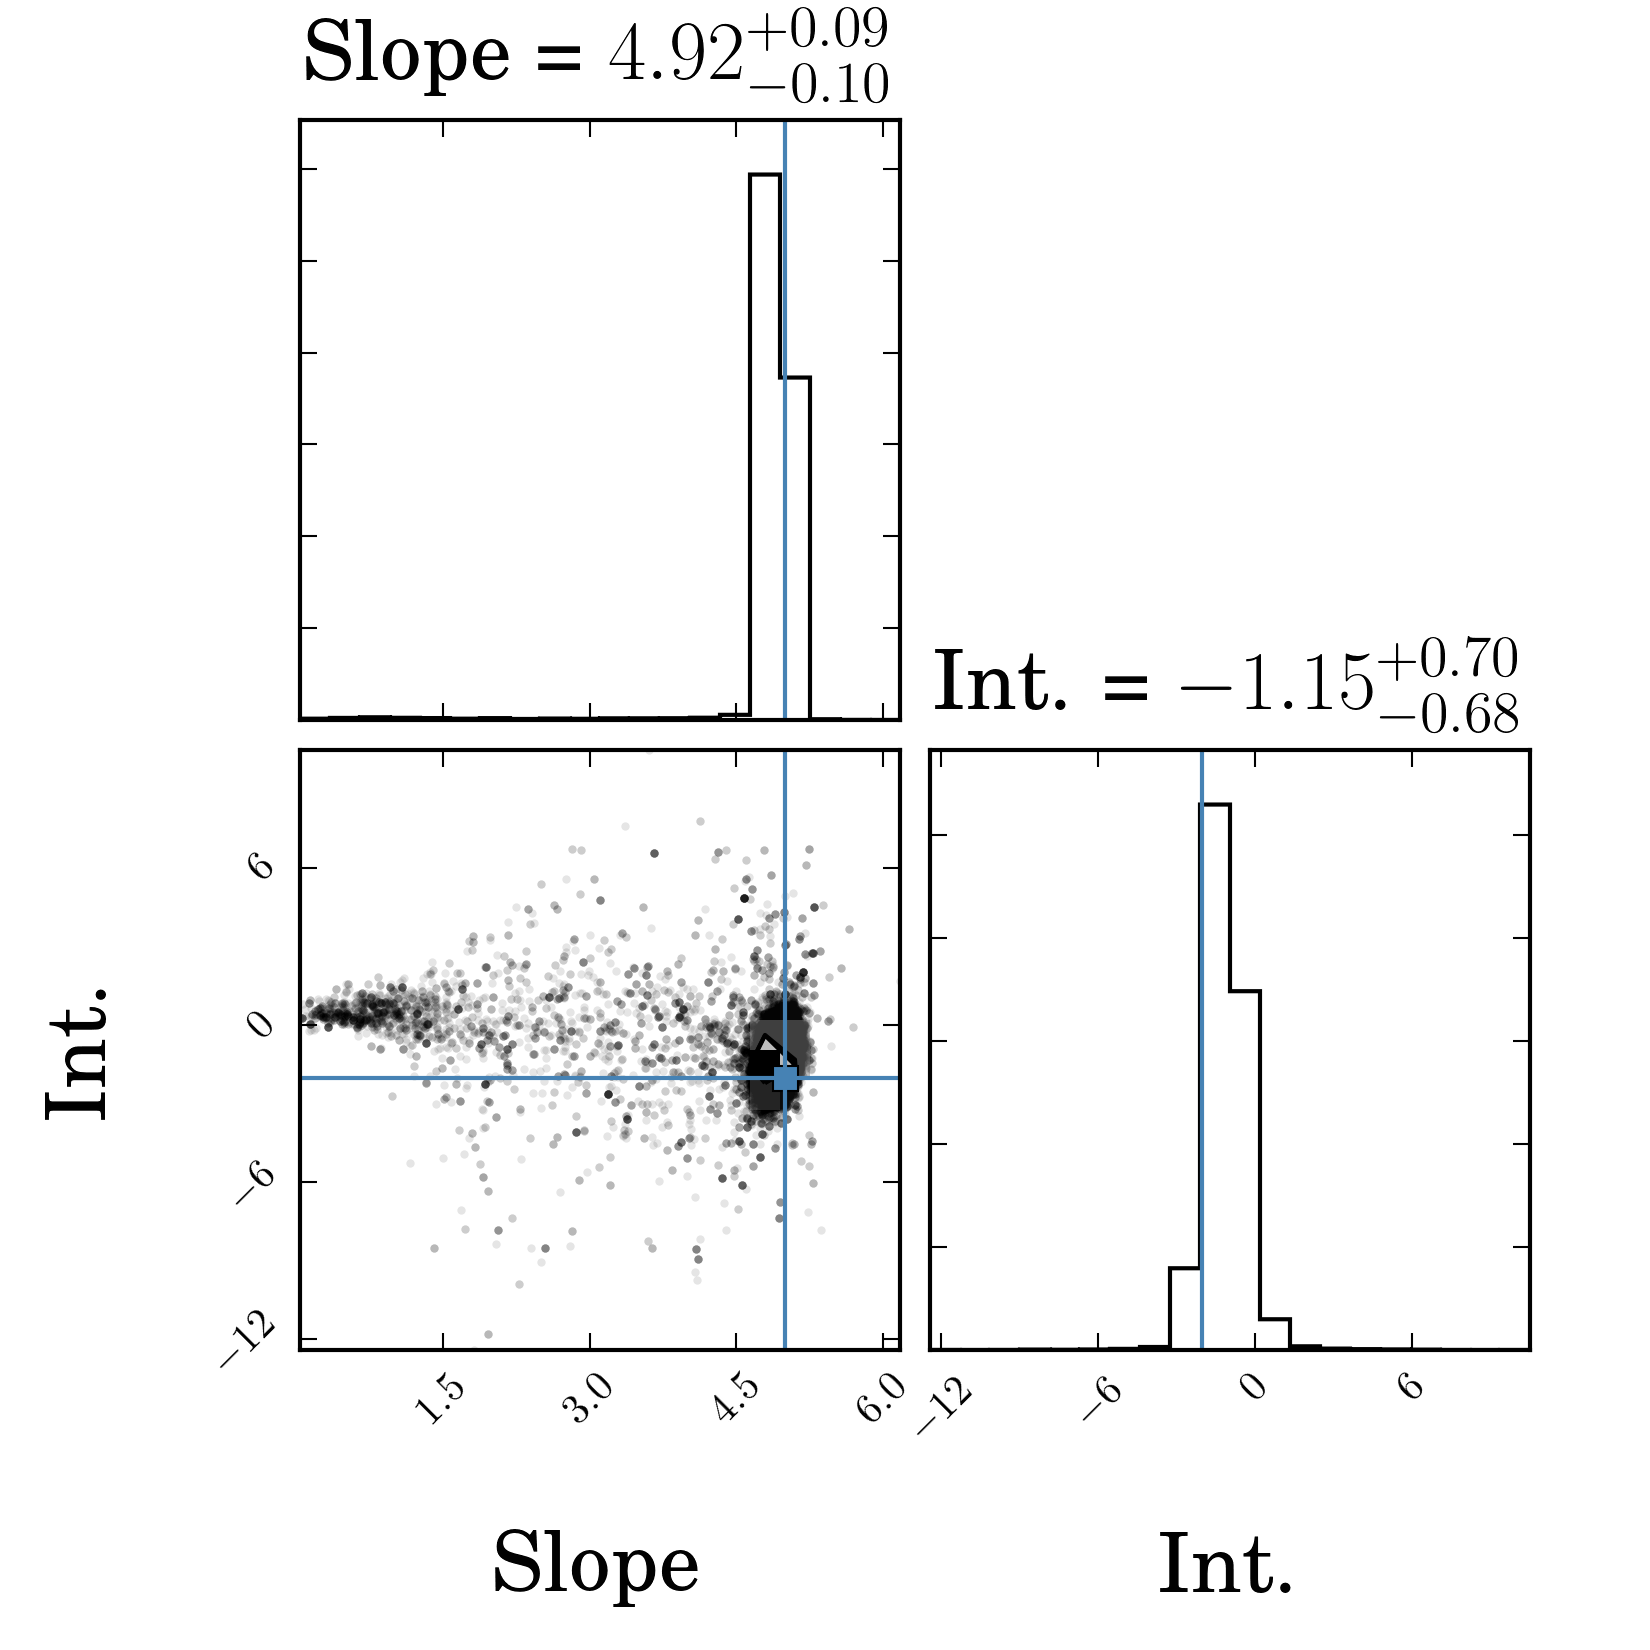
\includegraphics[width=\linewidth]{corner_10_data_points_emcee.png}
\endminipage\hfill
\minipage{0.32\textwidth}
  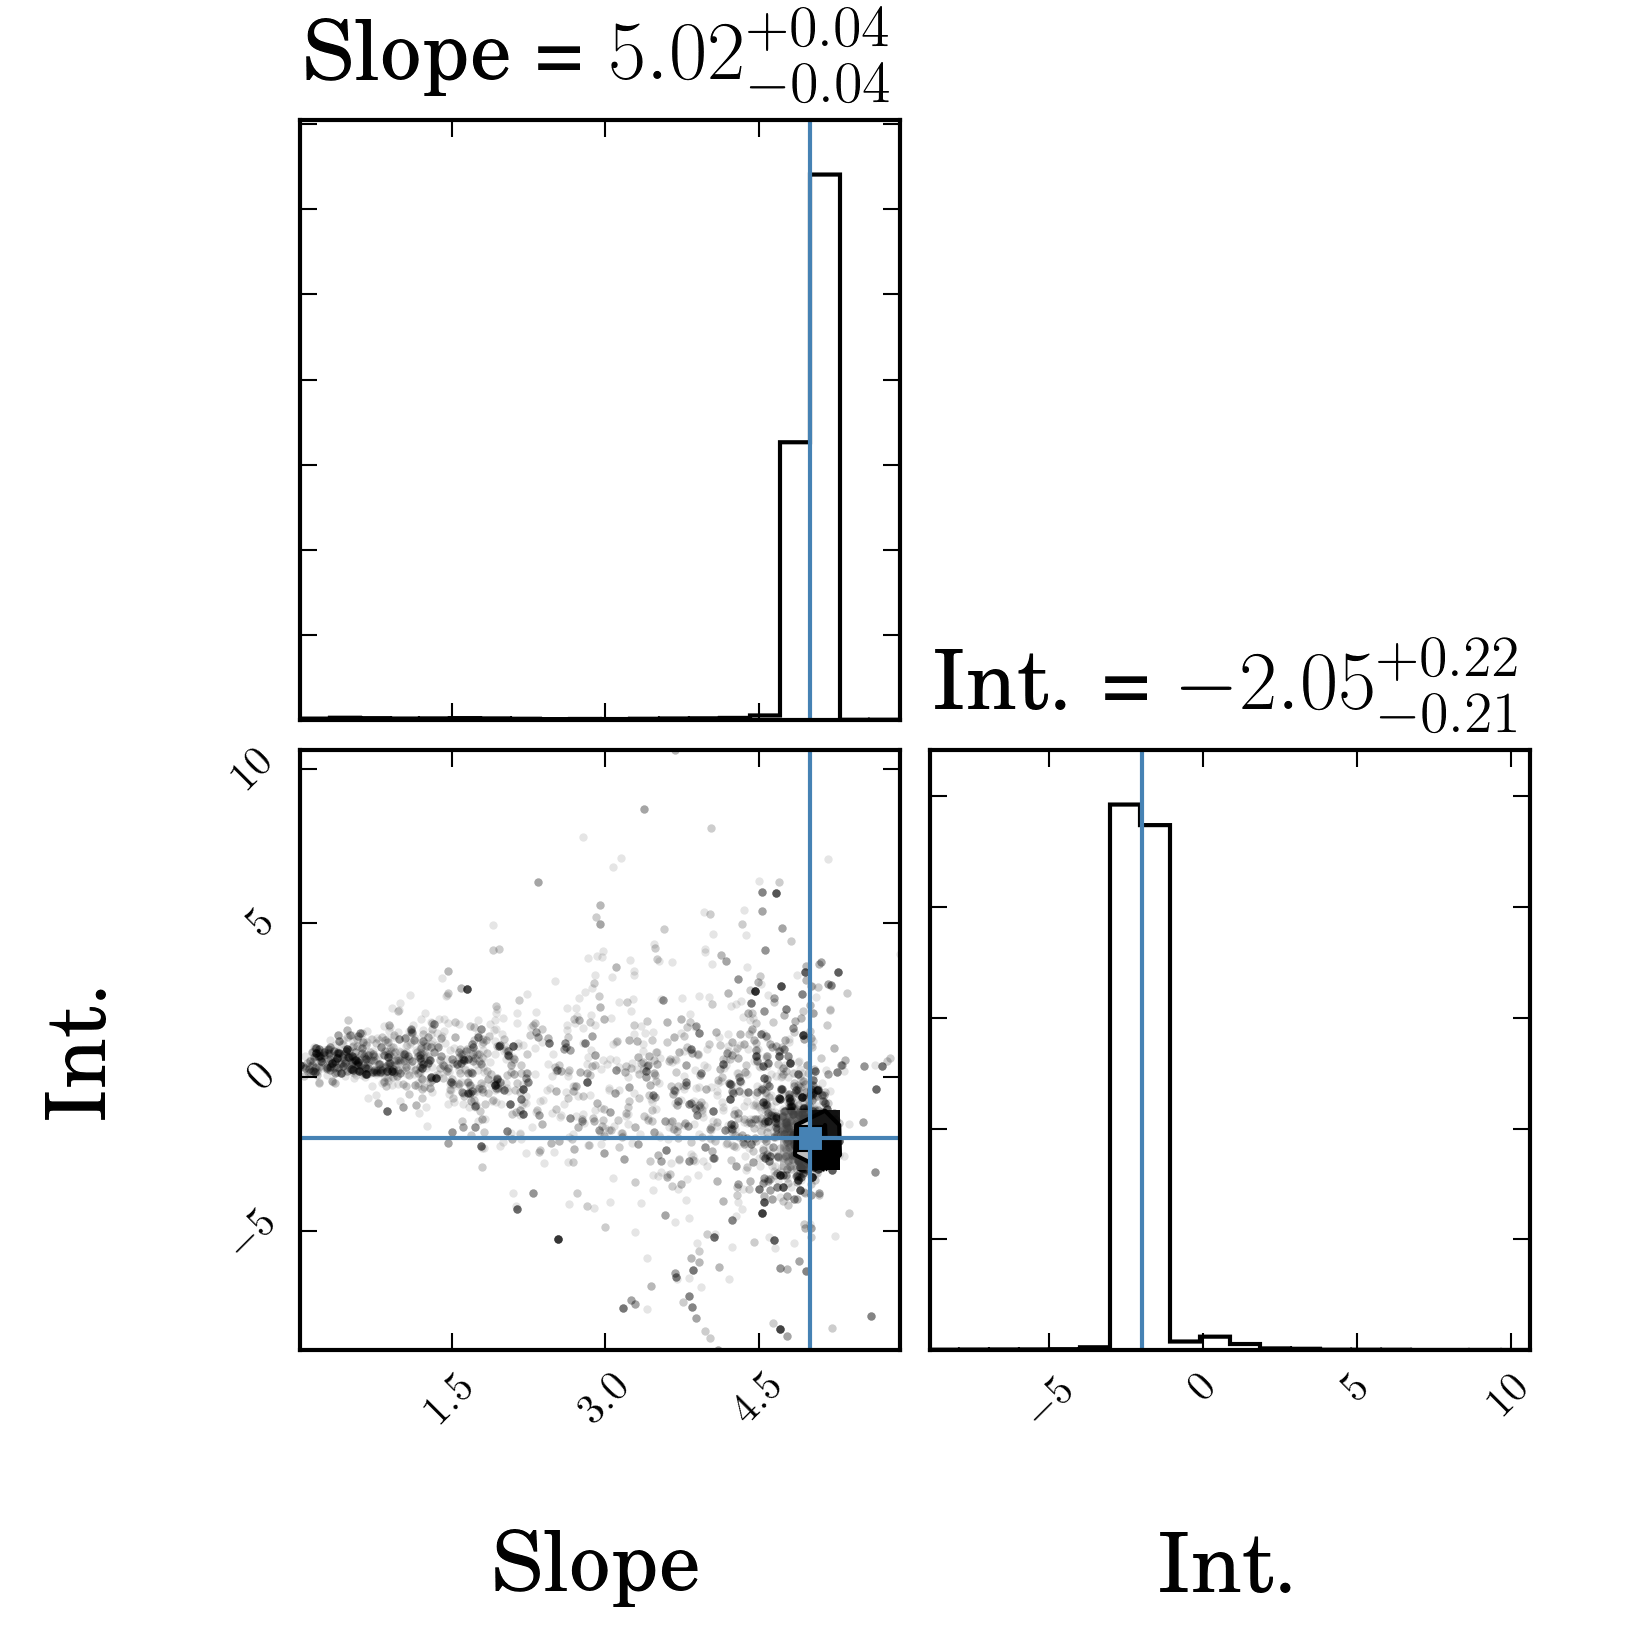
\includegraphics[width=\linewidth]{corner_100_data_points_emcee.png}
\endminipage\hfill
\minipage{0.32\textwidth}%
  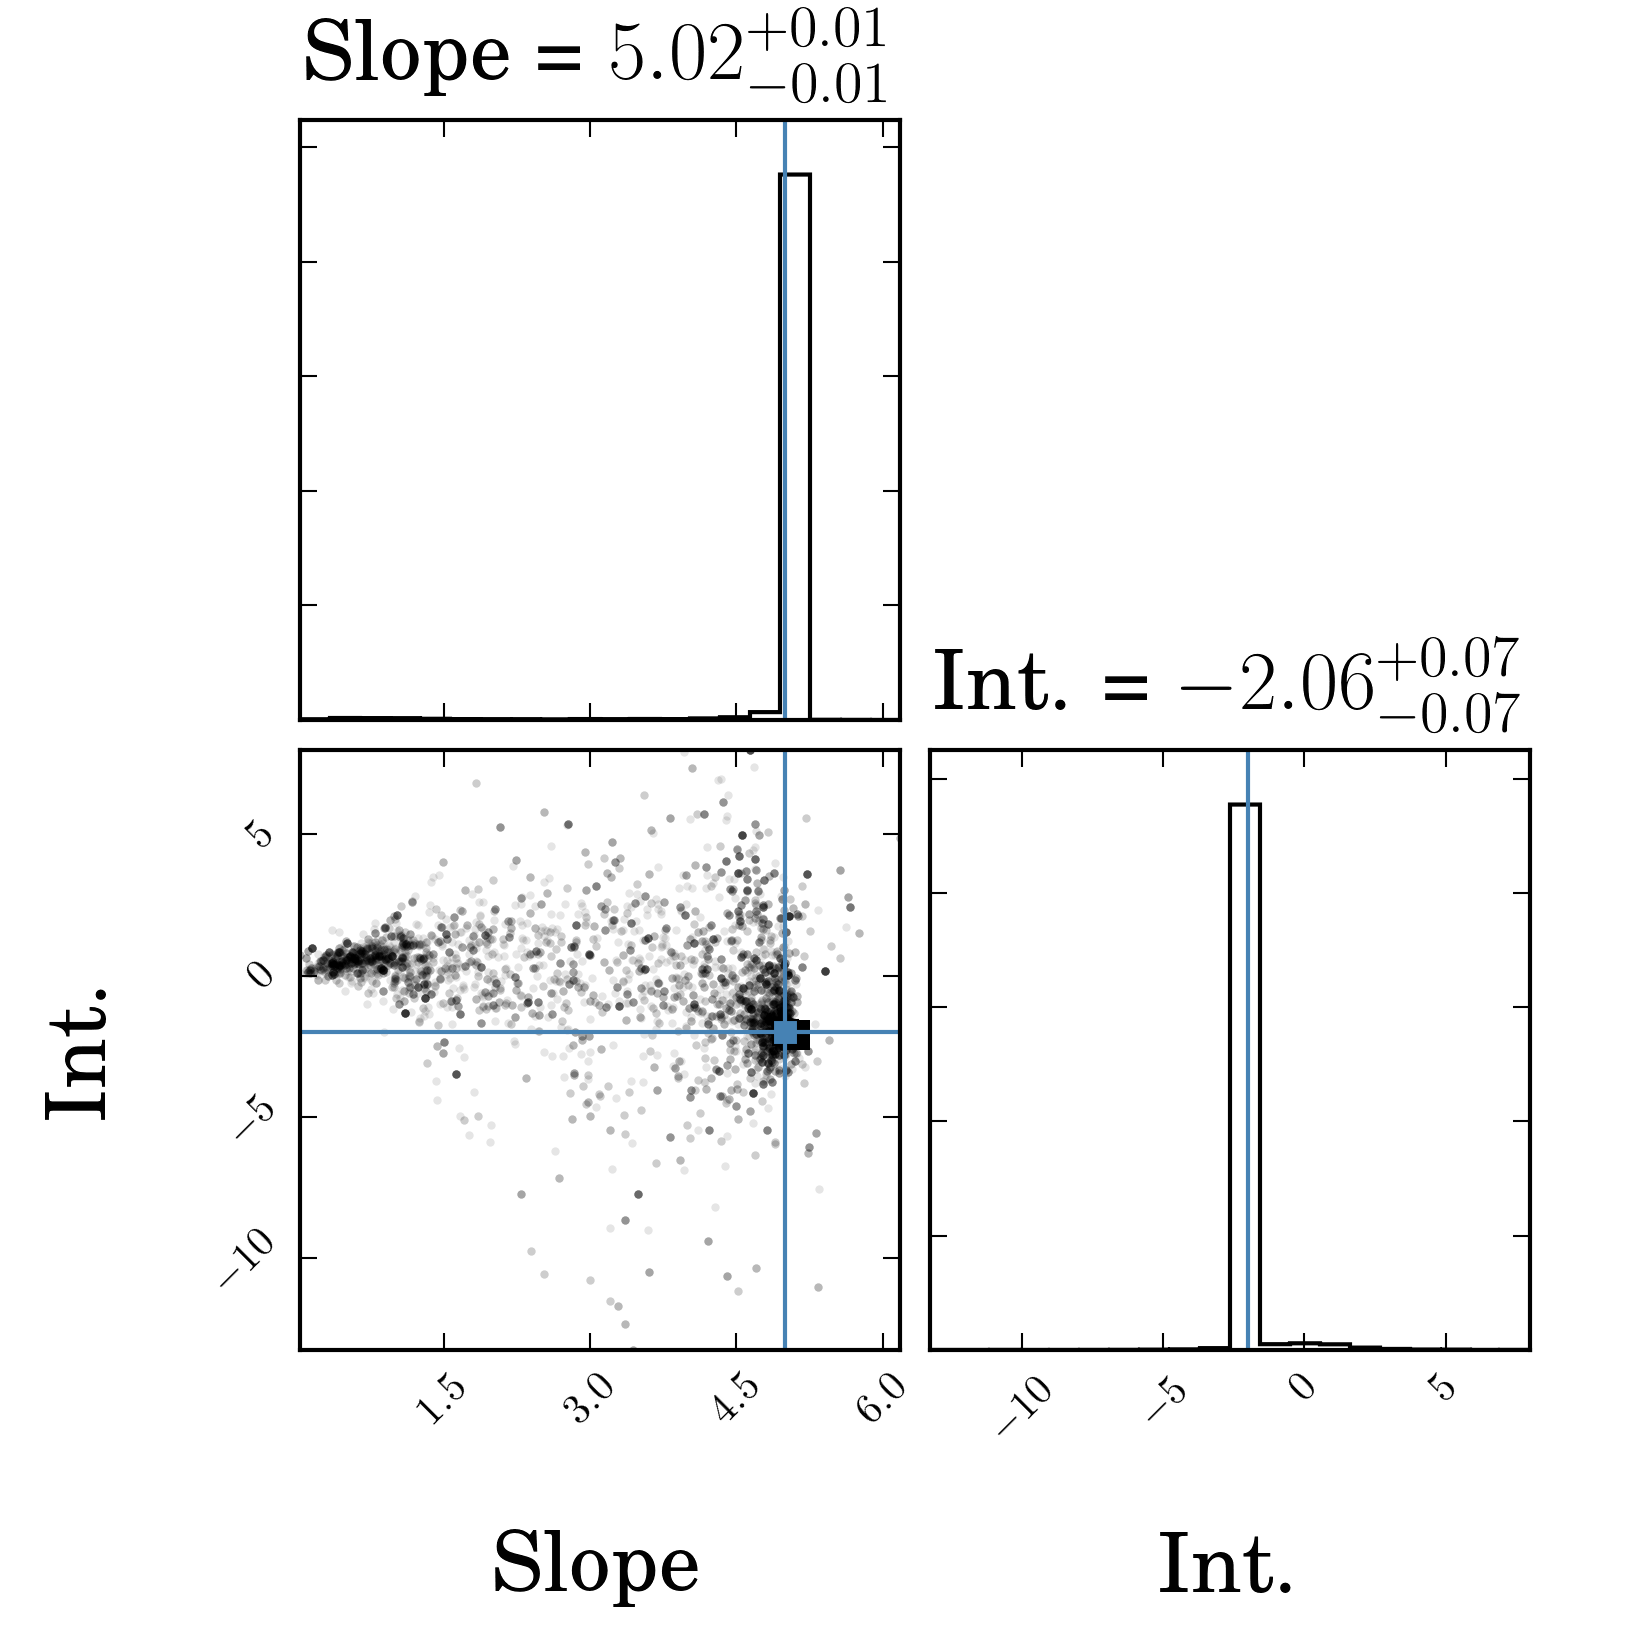
\includegraphics[width=\linewidth]{corner_1000_data_points_emcee.png}
\endminipage\hfill
\end{figure}

To reiterate, it is clear that emcee does a better job at finding more accurate and precise values of m and b than my own algorithm (which is definitely expected!). Additionally, emcee finds more accurate  and more precise values when the number of data points is higher-- evidenced by the narrowing of the peaks as you move right. As in the previous contours, the posterior curve for b is slightly broader than for m. 

Here are some diagnostic plots from the emcee run.


\begin{figure}[H]
\centering
\caption{ln(P) vs. Step Number for a 100 Point Fake Data Set from emcee}
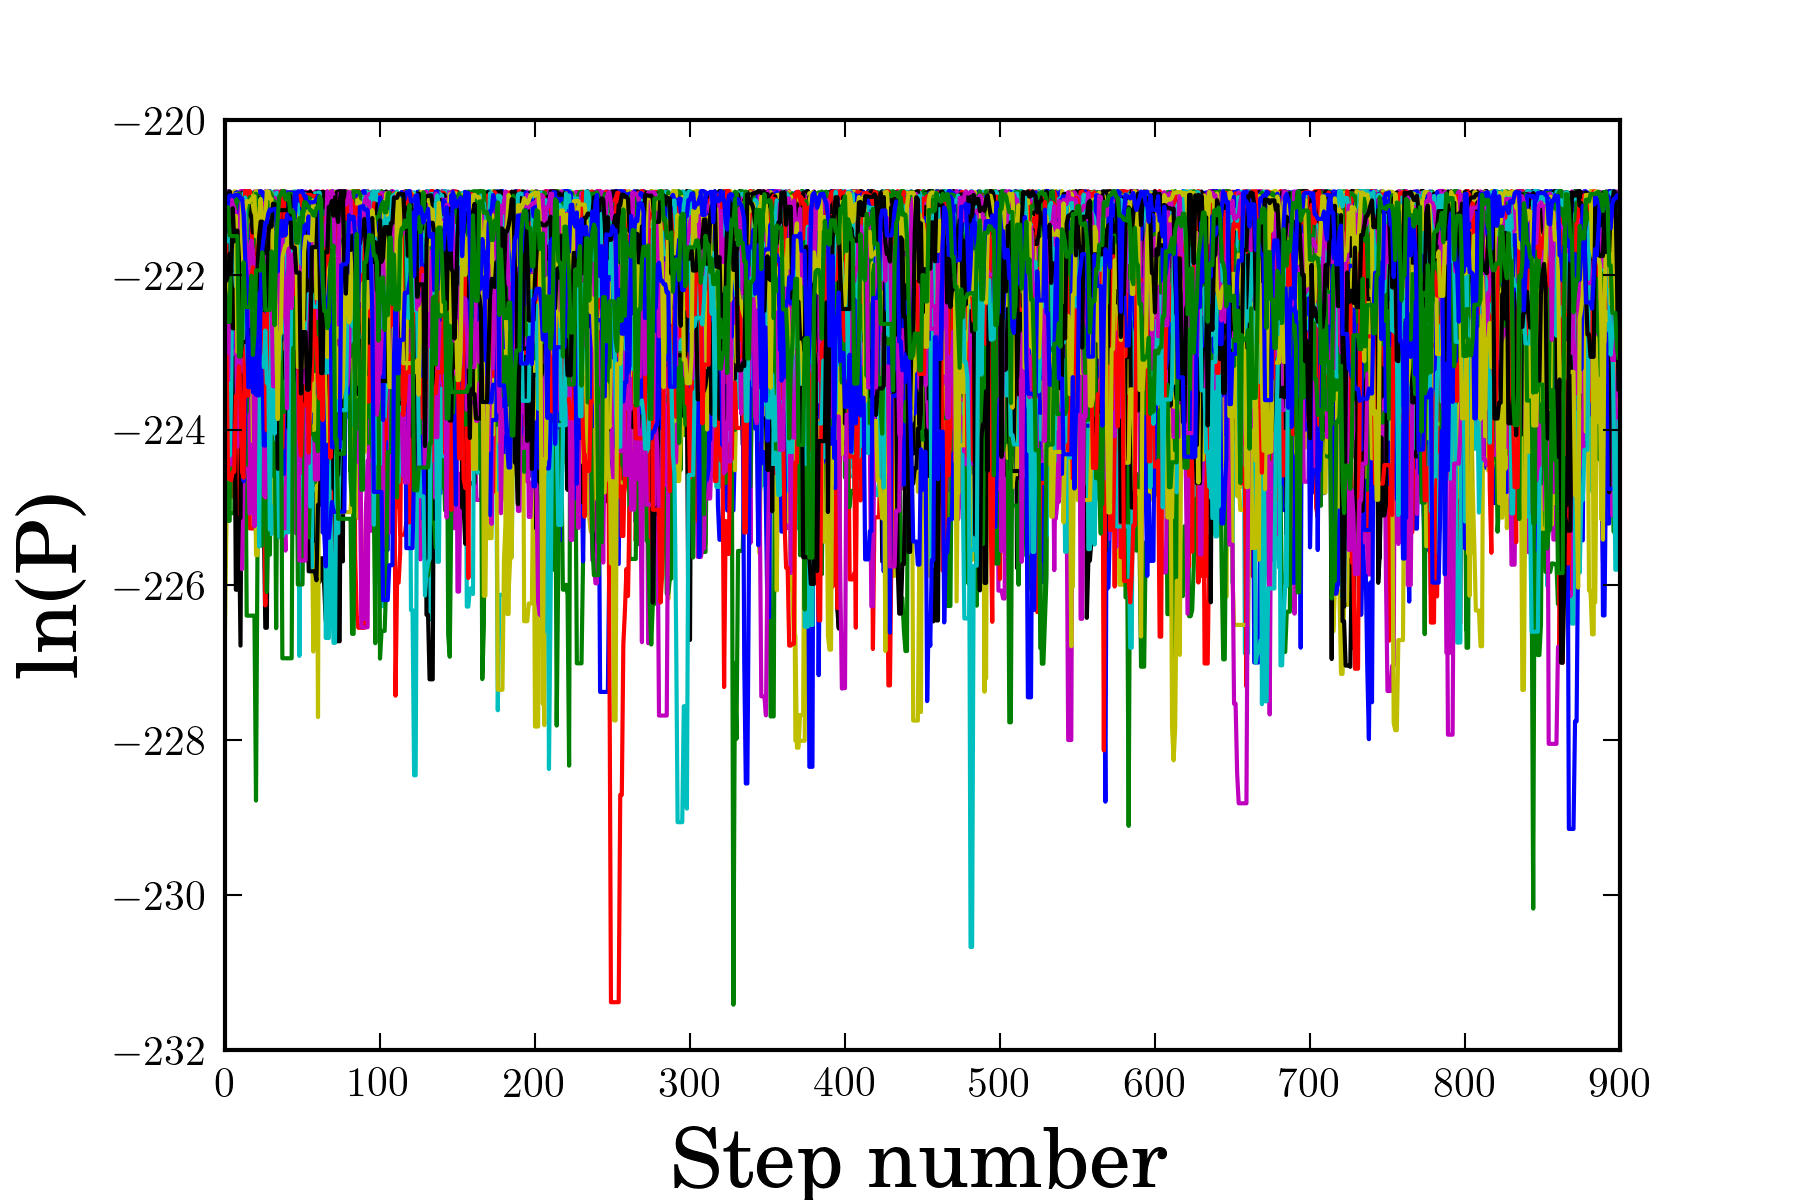
\includegraphics[scale = 0.6]{lnp_step_100_emcee.png}
\end{figure}


\begin{figure}[H]
\caption{These figures are from a 100 fake data point data set.}
\centering
\begin{subfigure}{.4\textwidth}
  \centering
  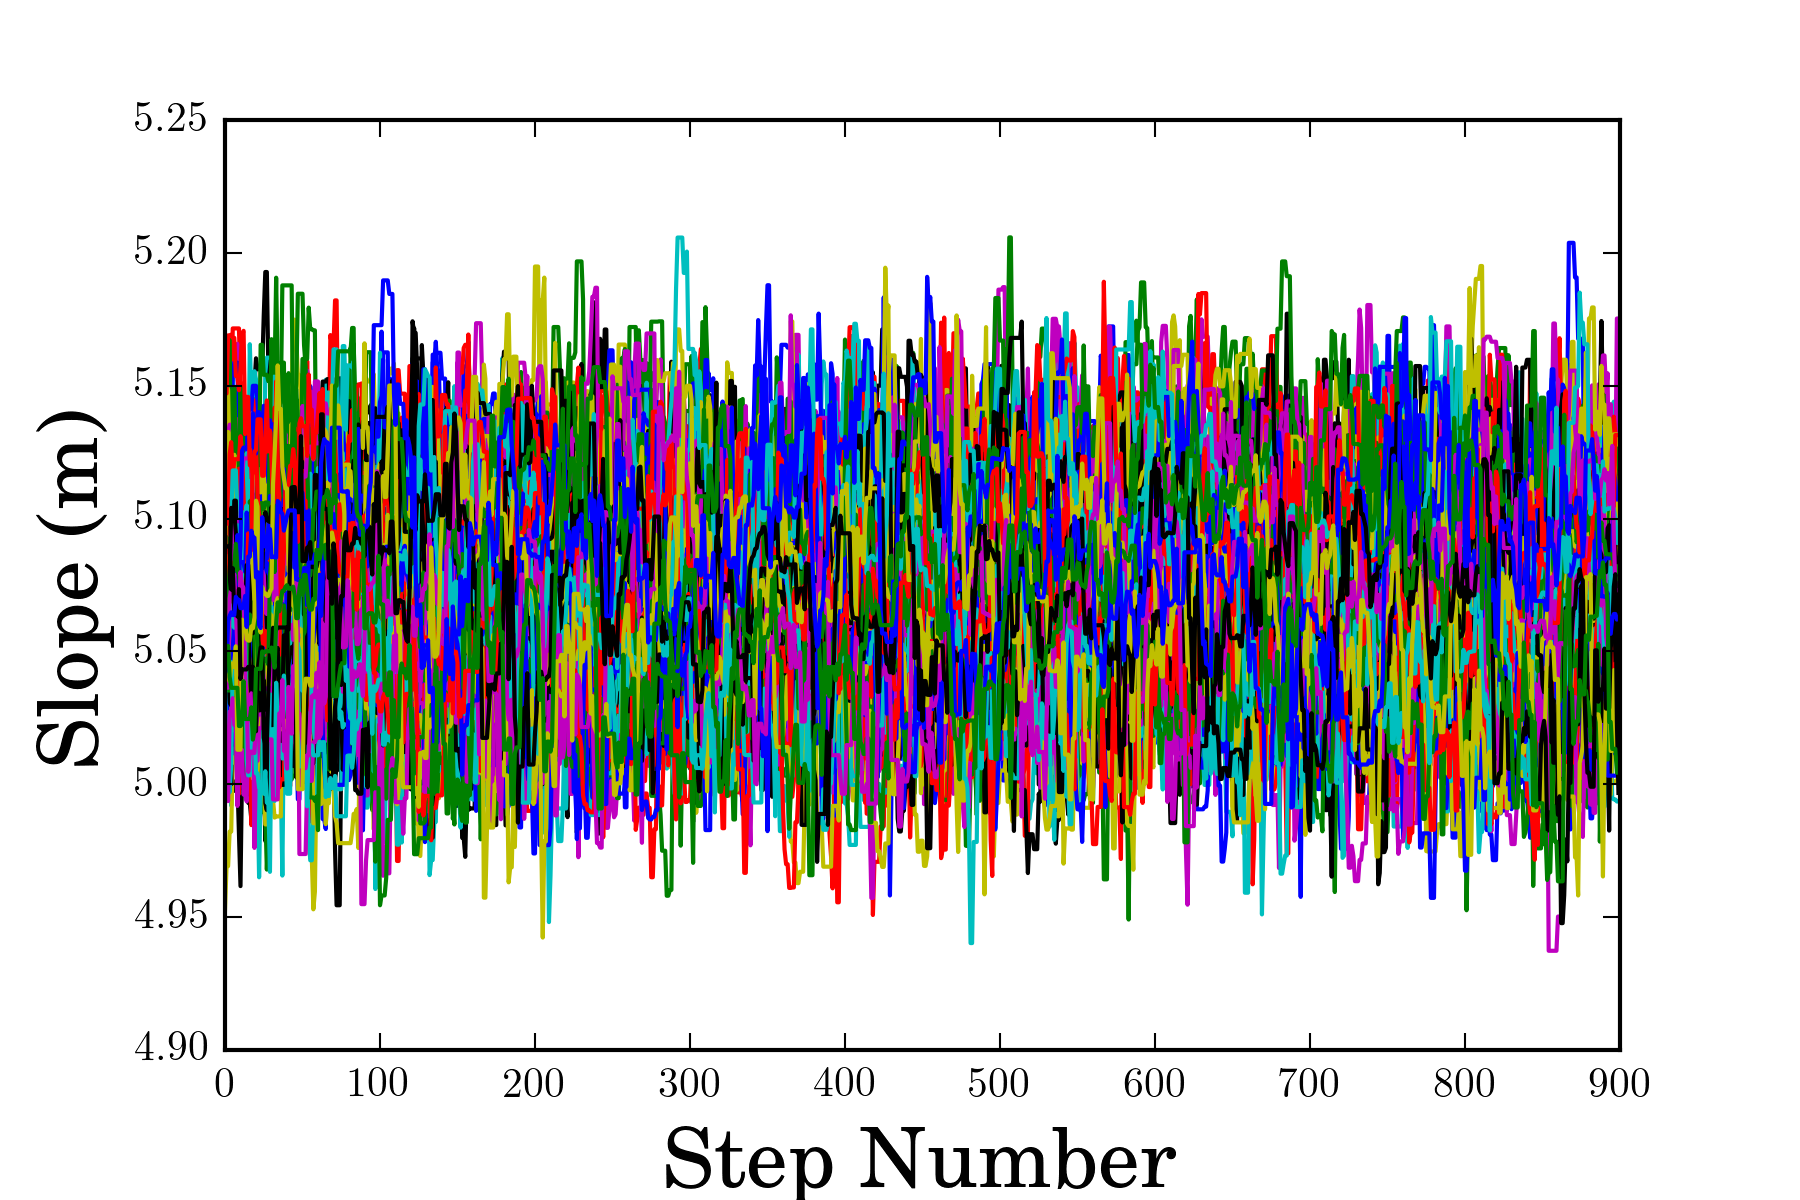
\includegraphics[width=\linewidth]{m_step_100_emcee.png}
  \caption{m vs. Step Number}
  \label{fig:sub1x}
\end{subfigure}%
\begin{subfigure}{0.4\textwidth}
  \centering
  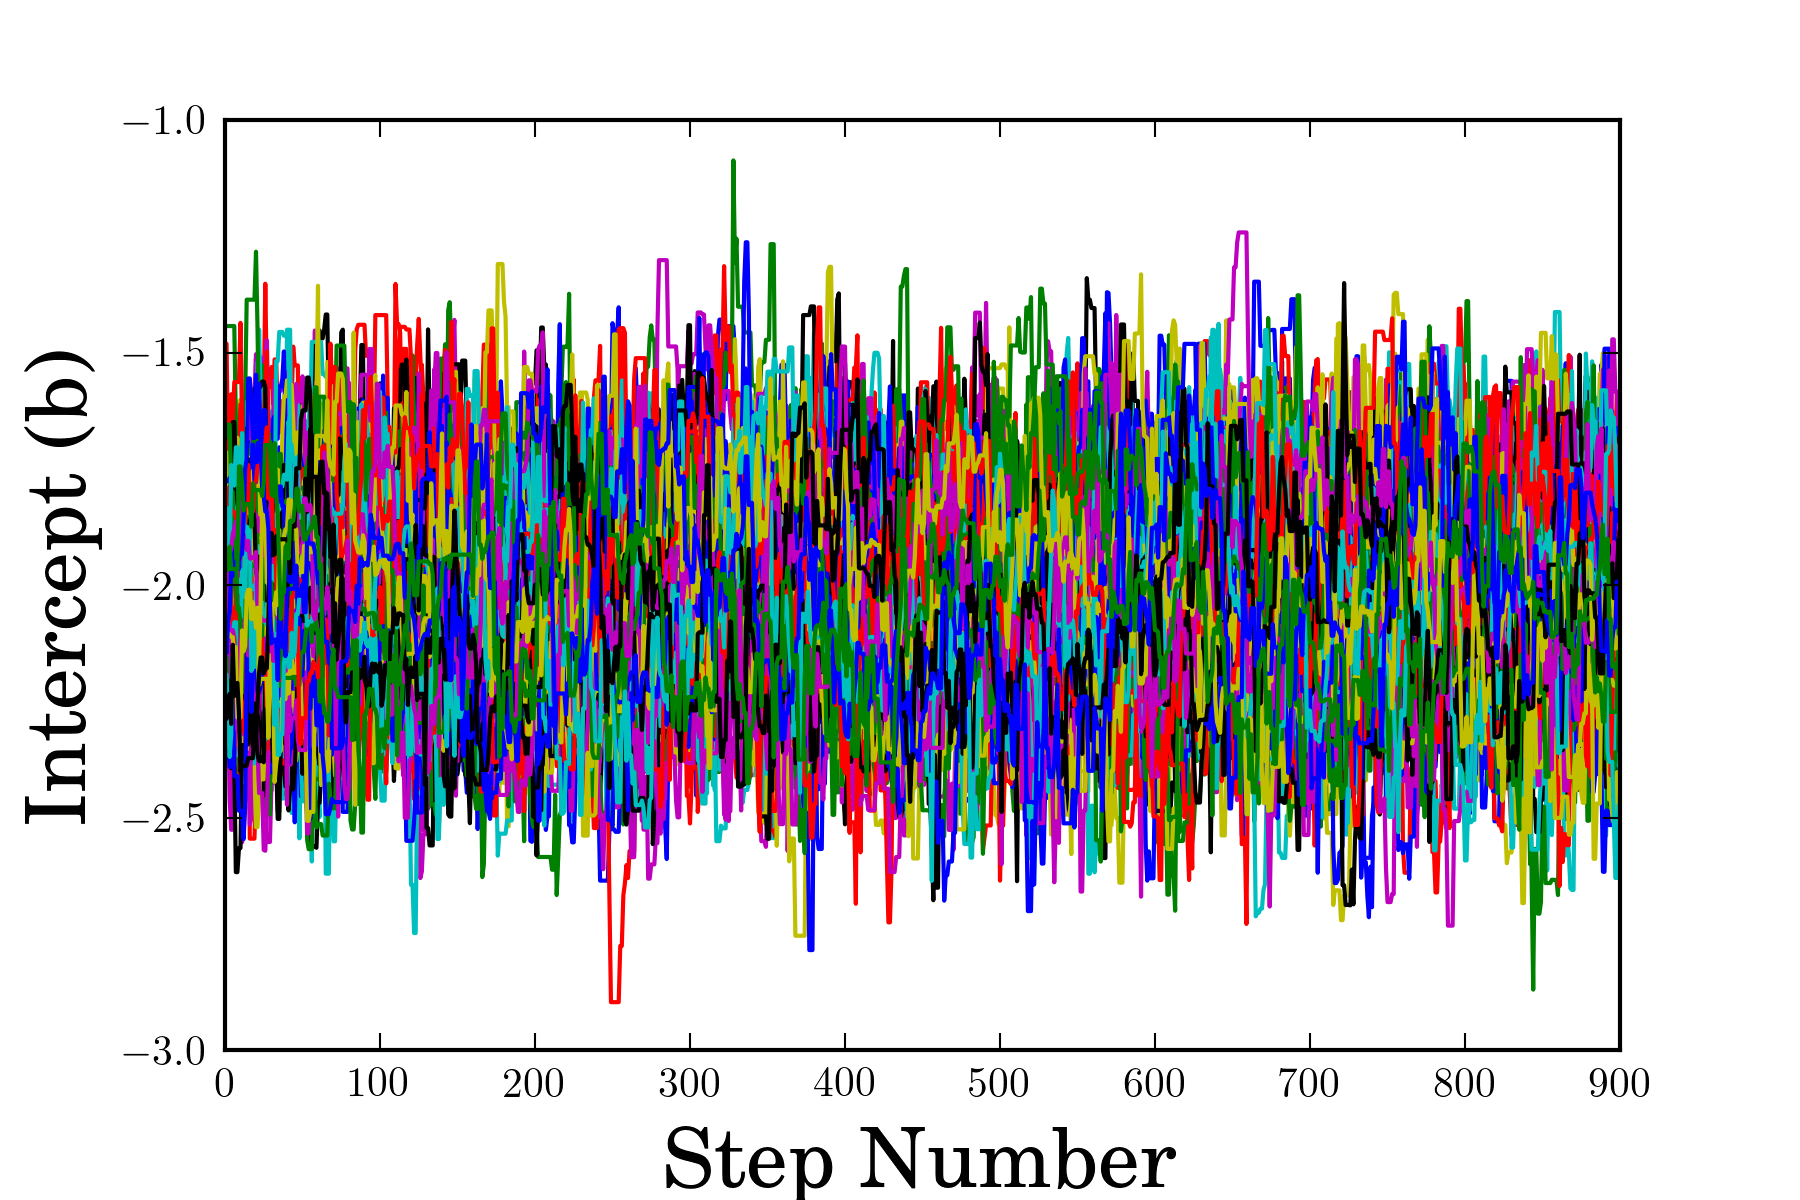
\includegraphics[width=\linewidth]{b_step_100_emcee.png}
  \caption{b vs. Step Number}
  \label{fig:sub2x}
\end{subfigure}
\label{fig:testx}
\end{figure}

After a burn in period, the chains appear to converge to fairly steady values. The above plots have the initial burn in portion of the chain removed. There are no clear trends in the data, which implies convergence.

\end{document}